
\subsection{Charged multiquark candidates $Z_{c}$ and $Z_{cs}$}

\subsubsection{$Z_{c}$ in $B$ decay }

The first candidate of charged charmonium-like state is $Z(4430)$,
which was observed at \belle in $\Bbar\to\psi\pip\Km$ decay in 2007\supercite{PhysRevLett.110.252001},
and in this plotthe signal structure is shown in the left of Figure.~\ref{fig:Z4430}.
Then the existence of $Z(4430)$ was independently confirmed in 2014 at \lhcb experiment\supercite{LHCb-PAPER-2014-014},
which was studied based on a 4-dimentional amplitude analysis in the $\Bbar\to\psi\pip\Km$ decay.
According to these independent measurements,
the average mass and width are determined to be $M=4478^{+15}_{-81} \mev$ and $\Gamma=181\pm31 \mev$ for $Z_{c}(4430)$.
Besides,
the $J^{P}$ assignment is ascertained to be $1^{+}$ at $9.7\sigma$ level as well.
The corresponding "Argand" plot is shown in the left of Figure.~\ref{fig:Z4430_argand},
revealing the character of Breit-Wigner resonances as a nearly circular in shape.
In addition,
a broad peak named as $Z_{c}(4240)$ is required for a satisfied fitting,
and this additional structure appeared in $\psi\pip$ mass distribution as shown in right of Figure.~\ref{fig:Z4430}.

\begin{figure}[!hbtp]
\centering
   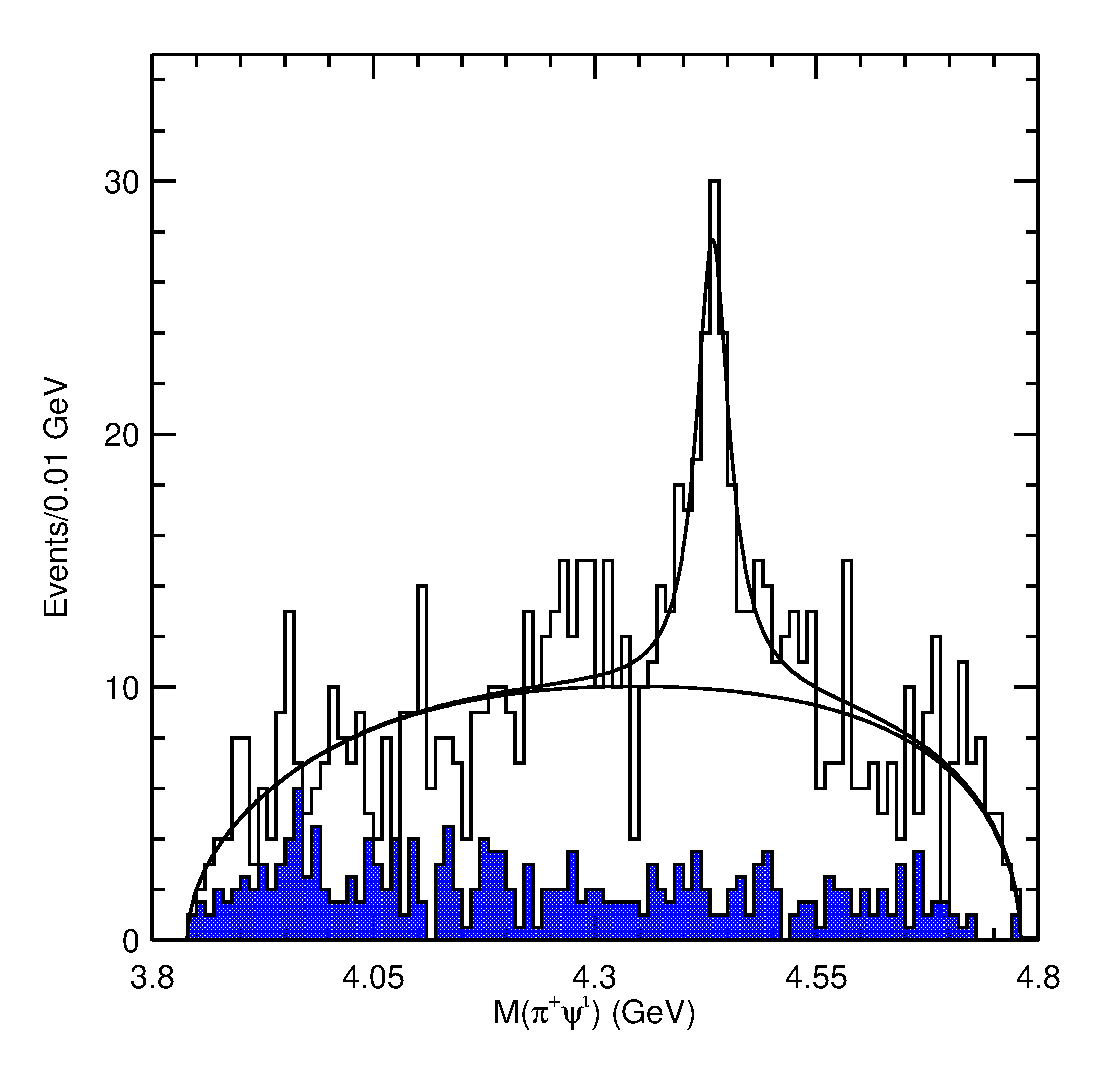
\includegraphics[width=0.43\textwidth]{Figures/01_Introduction/Exotic/charged_particle/Belle_Z4430} %
   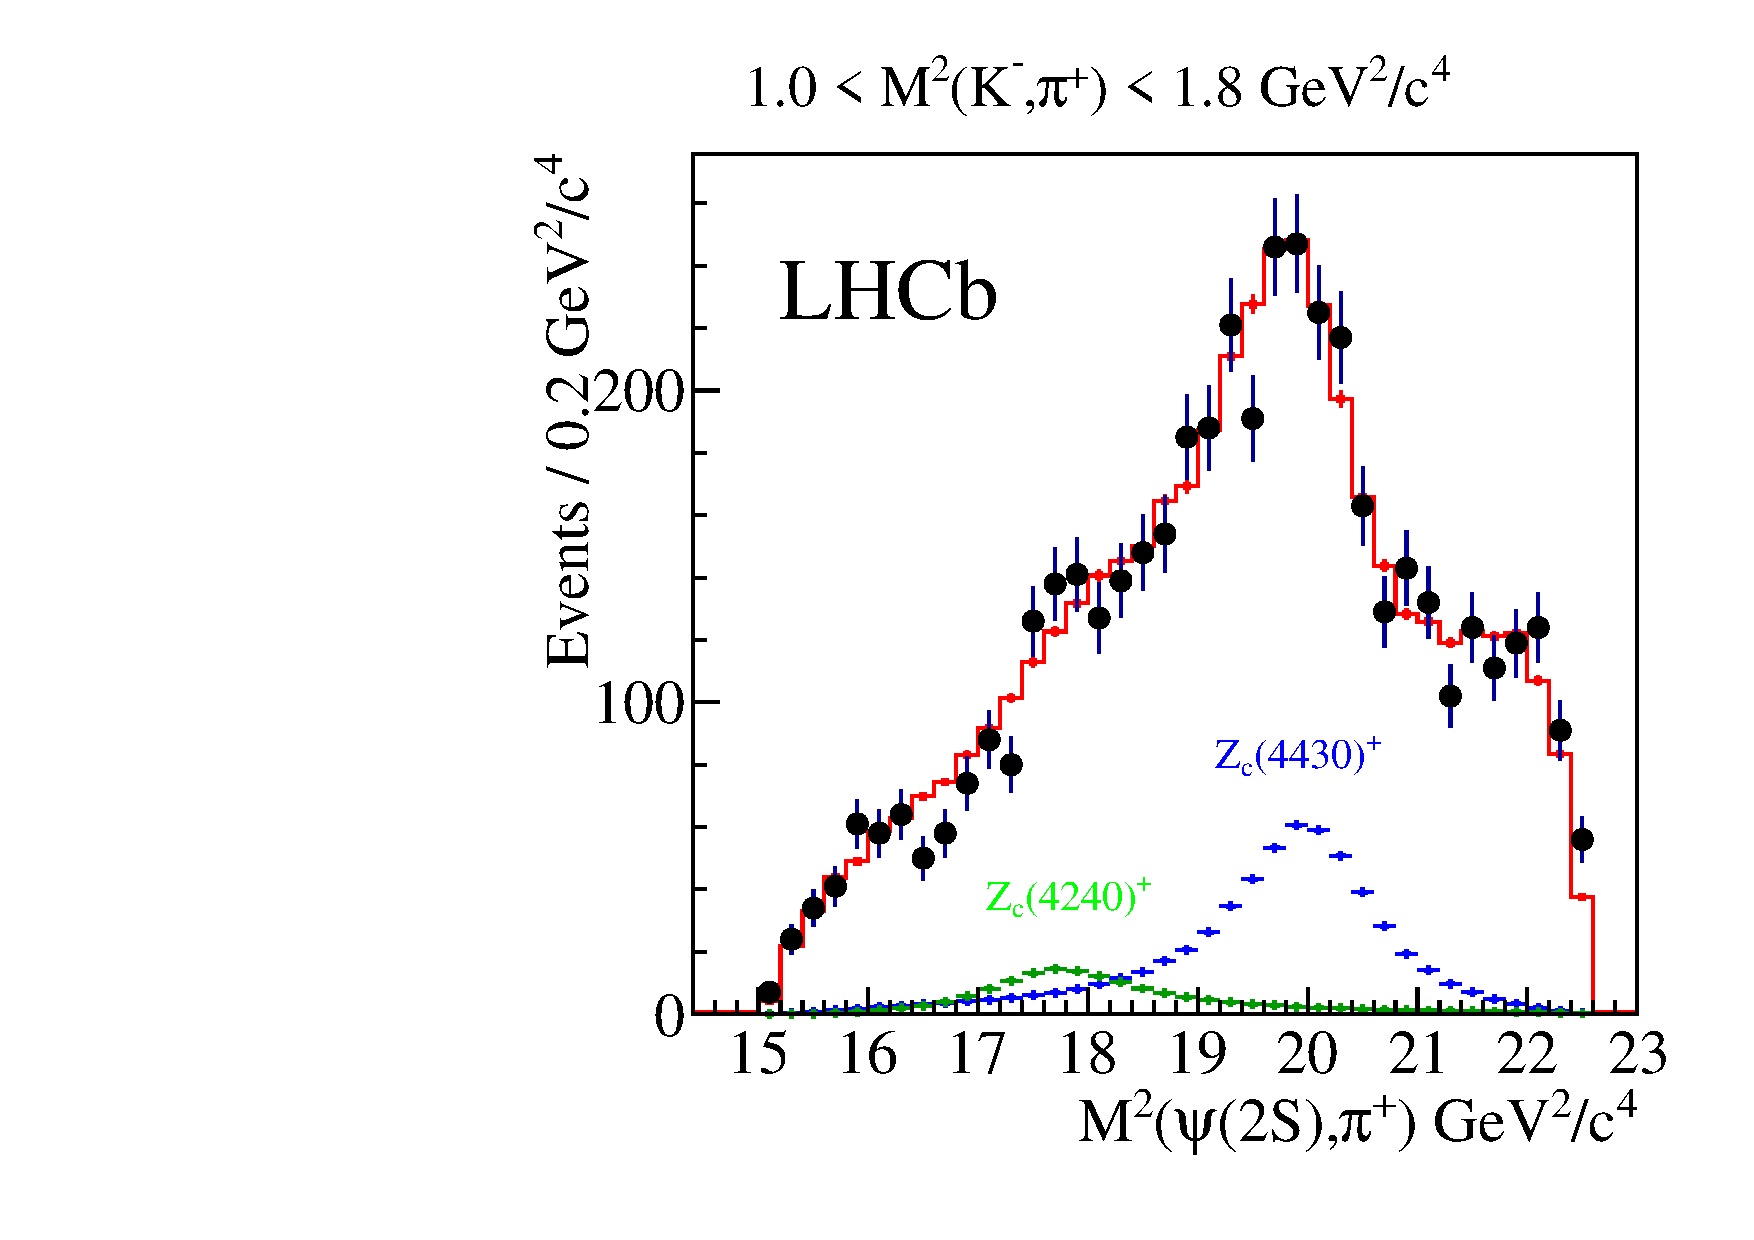
\includegraphics[width=0.46\textwidth]{Figures/01_Introduction/Exotic/charged_particle/LHCb_Z4430} %
   \caption{ 
   The $M(\psi\pi)$ distribution in $\Bbar\to\psi\pip\Km$ decay at \belle\supercite{PhysRevLett.110.252001},  
   the $M^{2}(\psi\pi)$ in $\Bbar\to\psi\pip\Km$ from \lhcb\supercite{LHCb-PAPER-2014-014}.}
\label{fig:Z4430}
\end{figure}


\begin{figure}[!hbtp]
\centering
   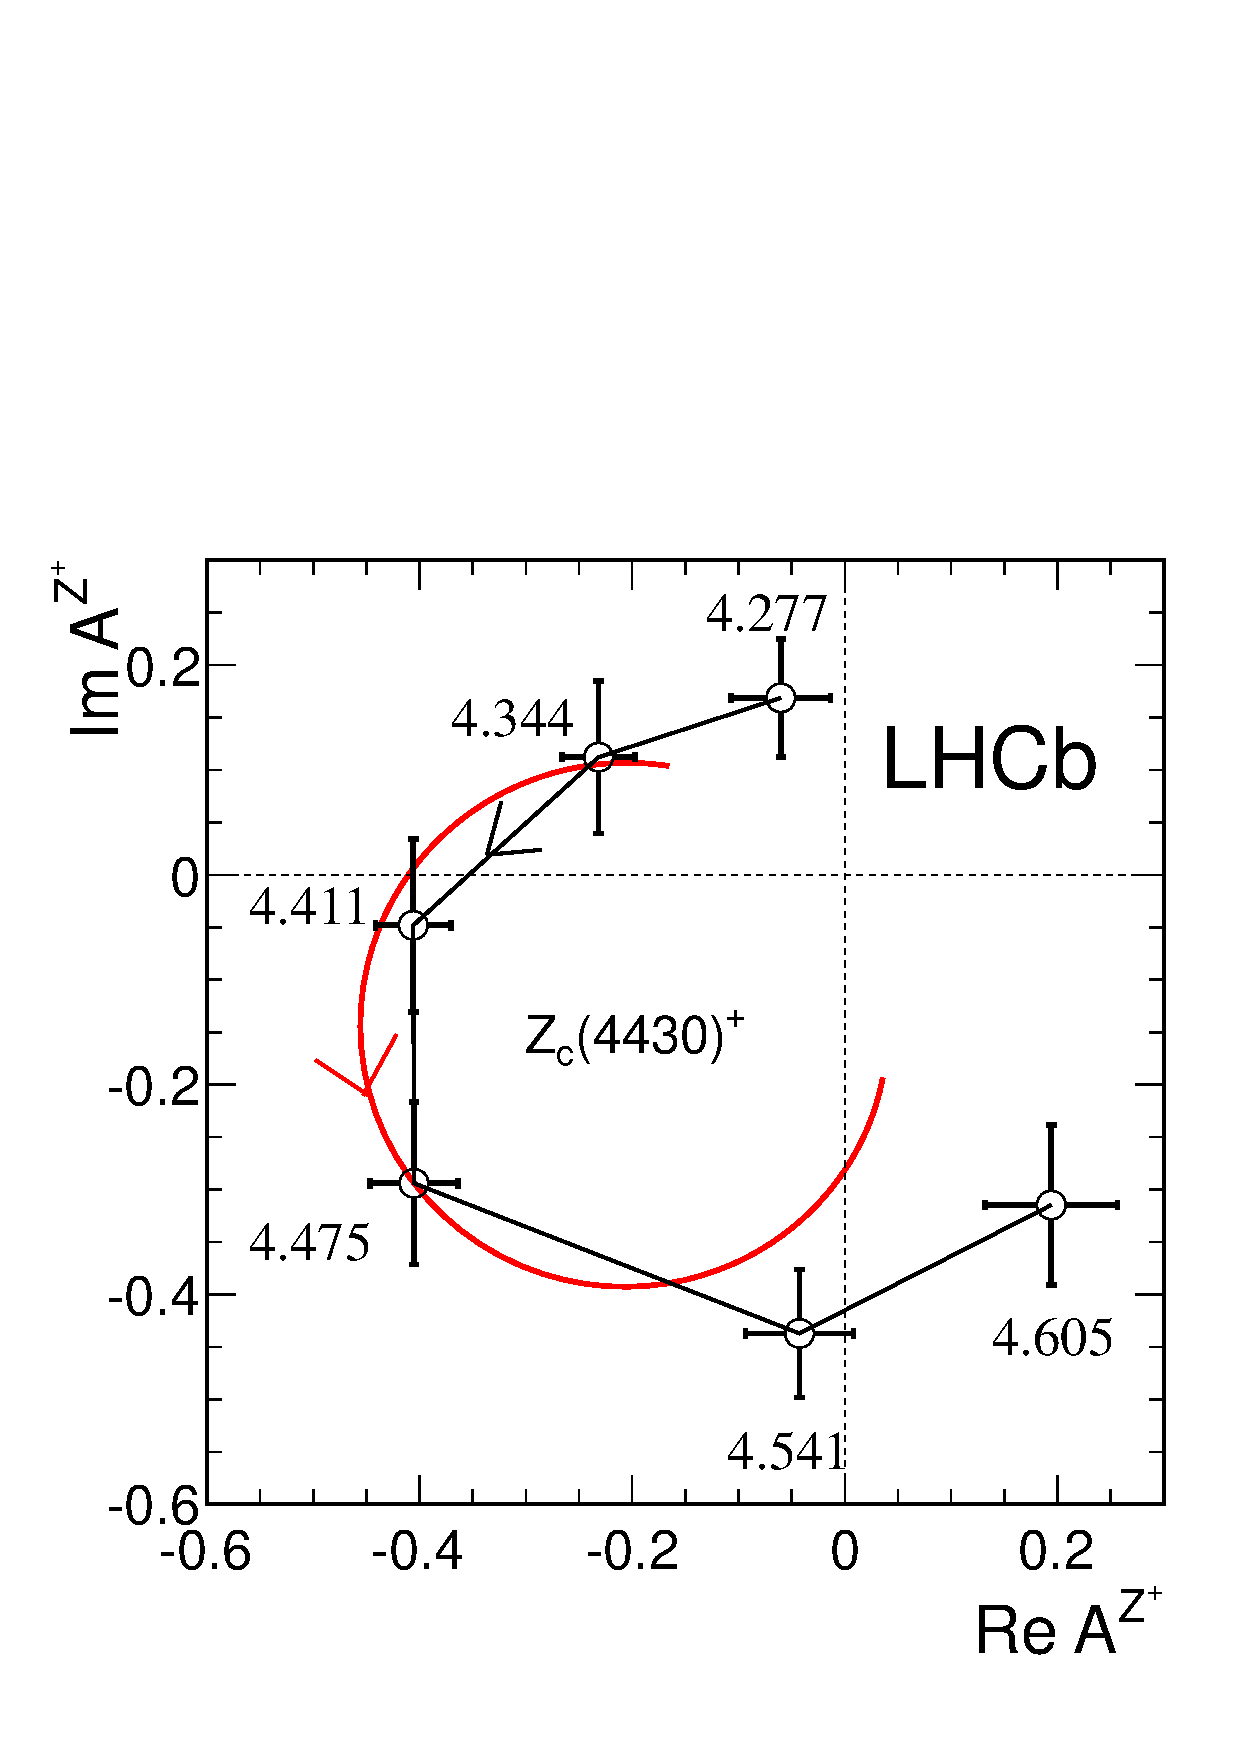
\includegraphics[width=0.4\textwidth]{Figures/01_Introduction/Exotic/charged_particle/Argand-Z} %
   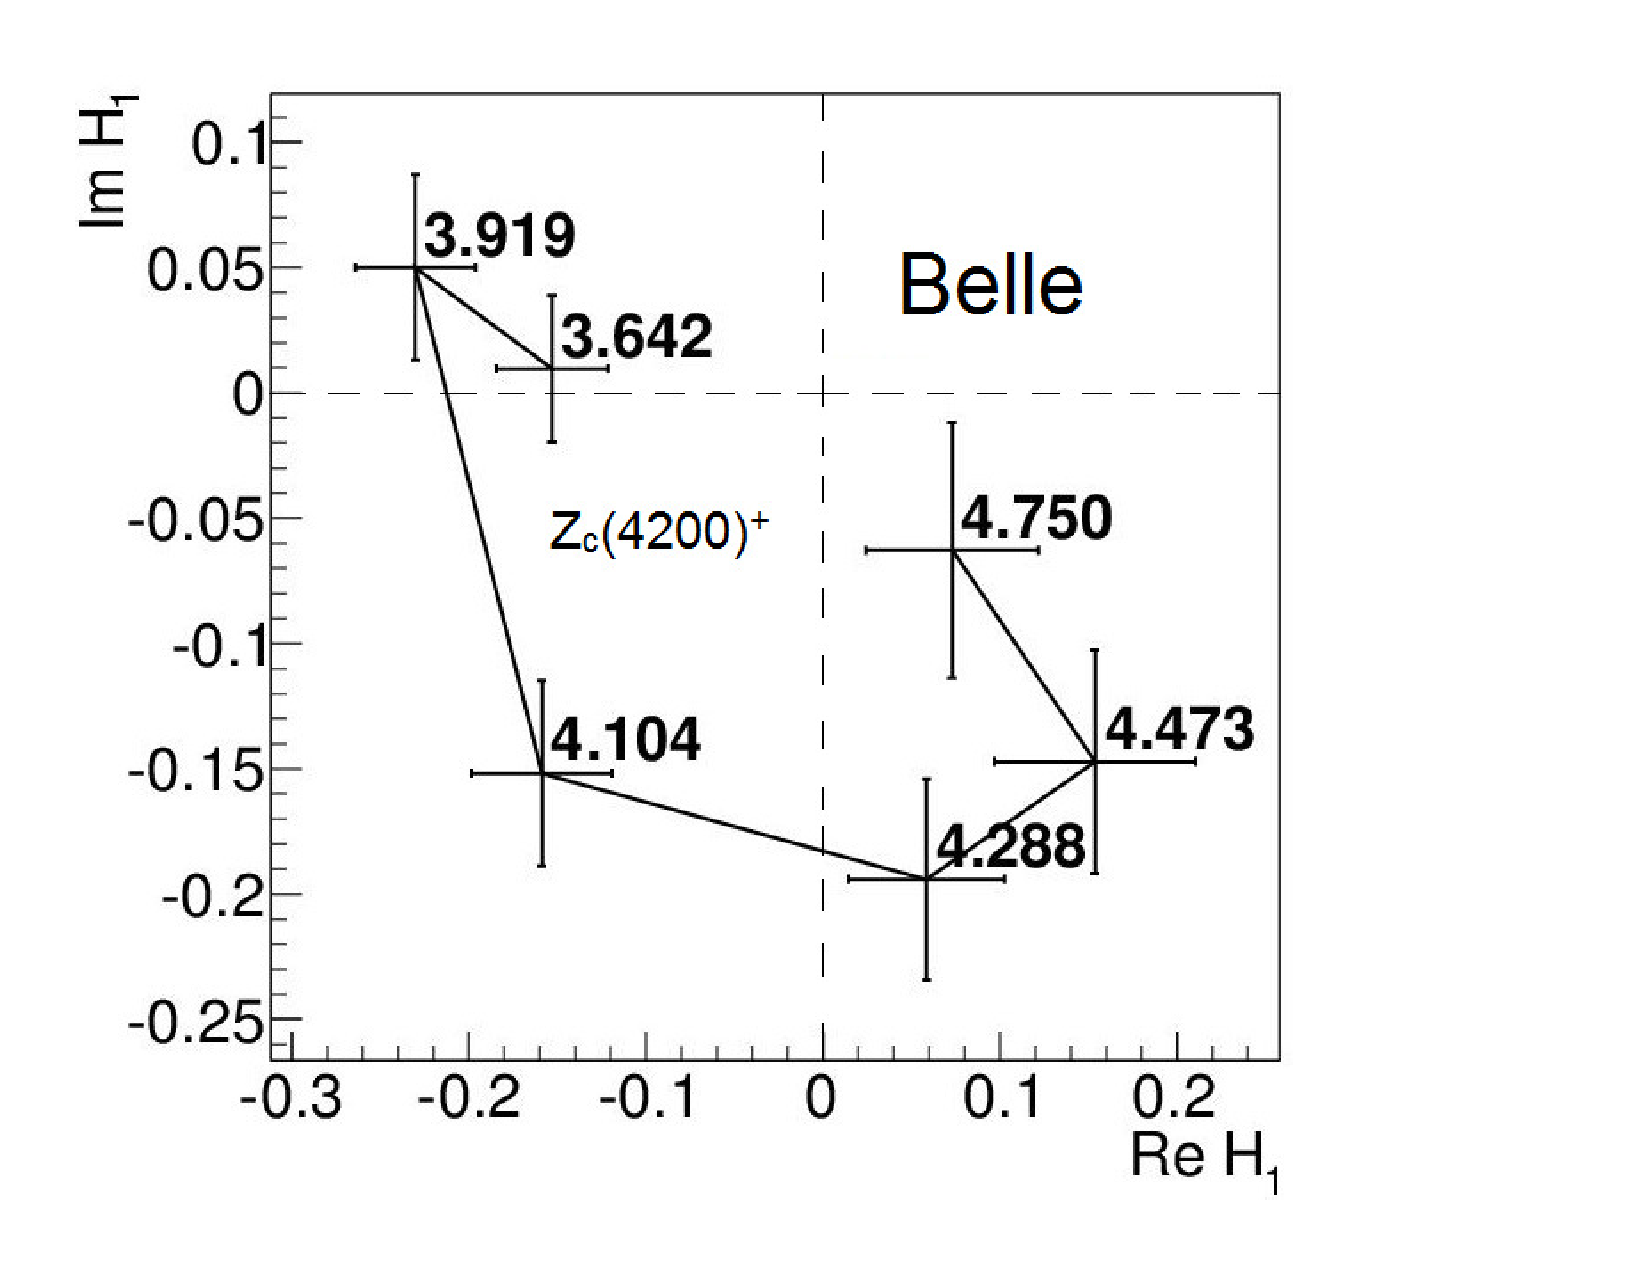
\includegraphics[width=0.52\textwidth]{Figures/01_Introduction/Exotic/charged_particle/Belle-Zc4200-Argand} %
   \caption{ 
   The real and imaginary parts of the amplitude for $Z_{c}(4430)\to\psi\pip$ decay at \lhcb\supercite{LHCb-PAPER-2014-014},  
   the $Z_{c}(4200)\to\jpsi\pip$ decay from \belle\supercite{PhysRevD.90.112009}.}
\label{fig:Z4430_argand}
\end{figure}

\belle also performed an amplitude of $\Bbar\to\jpsi\pip\Km$ decays\supercite{PhysRevD.90.112009},
and a new very broad $1^{+}$ $Z_{c}(4200)$ state is required for a satisfactory fit.
The measured mass and width of this state are $M=4196^{+31}_{-29}\pm^{+17}_{-13} \mev$ and $\Gamma=370\pm70^{+70}_{-132} \mev$.
Besides,
\belle also reported corresponding $J^{P}$ is either $0^{-}$ or $1^{+}$,
and "Argand" plot is shown in the right of Figure.~\ref{fig:Z4430_argand},
which displays a nearly circular phase motion.

The charged $Z_{c}$ states are pretty broad,
and the interference effect is very obvious, 
which can distort the resonance line shape.
For example,
the original $Z_{c}(4430)$ results were based on a one dimentional Breit-Wigner line-shape fit,
so they obtained lower values of mass and width than that from \lhcb.


\subsubsection{$Z_{c}$ in $\ep\en$ collision}

As mentioned in Section.~\ref{subsub:Y4260},
the $Y(4260)$ was observed at \babar.
This discovery prompted \besiii group to collect data at $E_{cm}=4260 \mev$ to search possible charged resonance 
in this channel.
%was excluded by \besiii.
Then,
the $Z_{c}(3900)$ was observed in $\jpsi\pip$ and $\jpsi\pim$ invariant mass distribution, 
using a 525 $\rm{pb^{-1}}$ \besiii data sample accumulatd at $E_{cm}=4.26\gev$\supercite{PhysRevLett.110.252001},
as shown in the left of Figure.~\ref{fig:3900}.
The measured mass is $3899.0\pm6.1 \mev$ and the width is $46\pm22$.
Significantly,
the mass of this state is around $24 \mev$ above the $m_{\Dstarp}+m_{\Dstarzb}$ threshold.
The $Z_{c}(3900)$ was observed by Belle at about the same time\supercite{PhysRevLett.110.252002}.

\begin{figure}[!hbtp]
\centering
   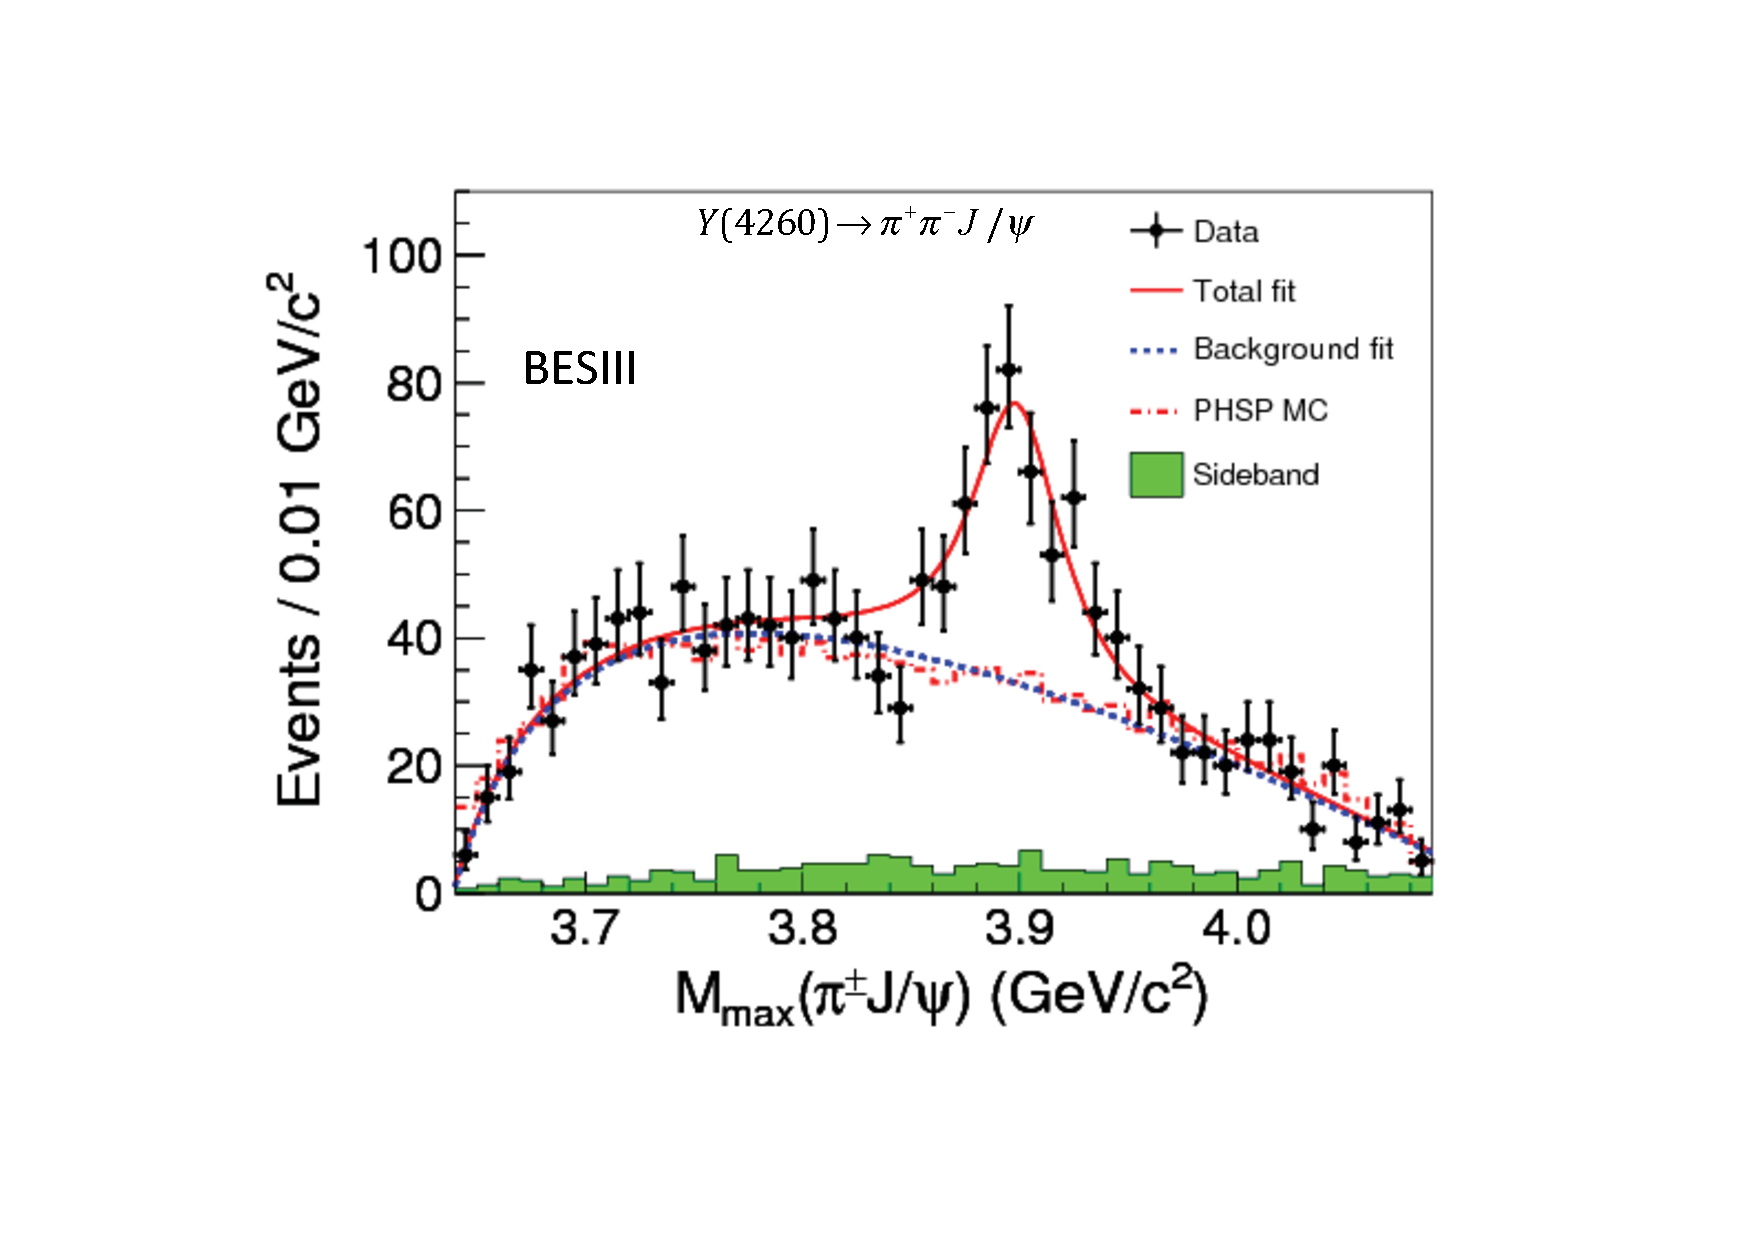
\includegraphics[width=0.43\textwidth]{Figures/01_Introduction/Exotic/charged_particle/bes3_zc3900} %
   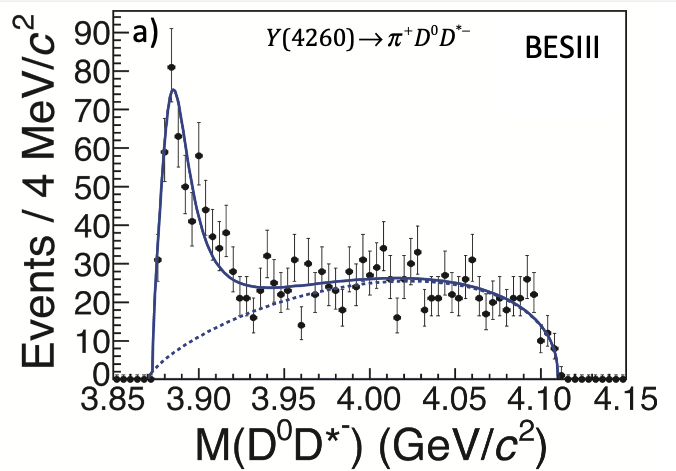
\includegraphics[width=0.46\textwidth]{Figures/01_Introduction/Exotic/charged_particle/bes3_Z3900_DD} %
   \caption{ 
   Distribution of the larger of two $\jpsi\pi^{\pm}$ masses in $\ep\en\to\jpsi\pip\pim$ events collected in \besiii
   at $E_{cm}=4260 \mev$\supercite{PhysRevLett.110.252001} (left),
   The $\Dz\Dstarm$ invariant mass distribution in $\ep\en\to\Dz\Dstarm\pip$ events collected in \besiii at $E_{cm}=4260 \mev$
   \supercite{PhysRevLett.112.022001} (right)}.
\label{fig:3900}
\end{figure}

Subsequently,
\besiii explored the $\Dz\Dstarm$ invariant mass distribution in $\ep\en\to\Dz\Dstarm\pip$ events,
and found the very strong near-threshold peak in this distribution,
as shown in the right of Figure.~\ref{fig:3900}.
Then the mass and width are determined as $M=3883.9\pm4.5 \mev$ and $\Gamma=24.8\pm12 \mev$ from a one-dimentional fit,
where the peak was discribed by a threshold-modified BW amplitude 
and background was repesented by a incoherent phase-space-like function\supercite{PhysRevLett.112.022001}.
Thus, 
this state was named as $Z_{c}(2885)$ by \besiii collaboration.
From the $Z_{c}(2885)\to\D\Dstarb$ stong decay,
\besiii also determined the $J^{P}$ quantum number to be $1^{+}$,
which is prefered than the $0^{-}$ or $1^{-}$ assignments.
\besiii also reported the observation of isospin partner of $Z_c(3900)$ in $\ep\en\to\jpsi\piz\piz$ events\supercite{PhysRevLett.115.112003},
as well as in $\ep\en\to\Dp\Dstarm\piz$\supercite{PhysRevLett.112.022001},
with mass and width are consistent with the charged $Z_{c}(3900)$ state.


In addition to $Z_c(3900)$,
\besiii collaboration observed the $Z_c(4020)$ in $h_c(1P)\pip\pim$ final states\supercite{PhysRevLett.111.242001},
and the invariant mass distribution of $h_{s}\pi^{\pm}$ is shown in the left of Figure.~\ref{fig:Z4020}.
In this study,
the mass of $Z_c(4020)$ was measured to be $4022.9\pm2.8 \mev$,
which is about $5 \mev$ above $m_{\Dstarp}+m_{\Dstarzb}$.
Similar to the neutral $Z_c(3900)$ study,
the isospin partner of $Z_c(4020)$ was searched in $\ep\en\to h_{c}\piz\piz$ events\supercite{PhysRevLett.113.212002},
as shown in the right of Figure.~\ref{fig:Z4020}.
Afterwards,
$Z_c(4020)$ and its isospin partner were searched in $\ep\en\to\Dstarp\Dstarz\pim$\supercite{PhysRevLett.112.132001} 
and $\ep\en\to\Dstar\Dstarzb\piz$\supercite{PhysRevLett.115.182002} events by \besiii. 
The measured mass and width from the double \D invariant mass spectrum are agree with those measured 
for the $Z_c(4020)\to h_{c}\pip$ channel within errors.

\begin{figure}[!hbtp]
\centering
   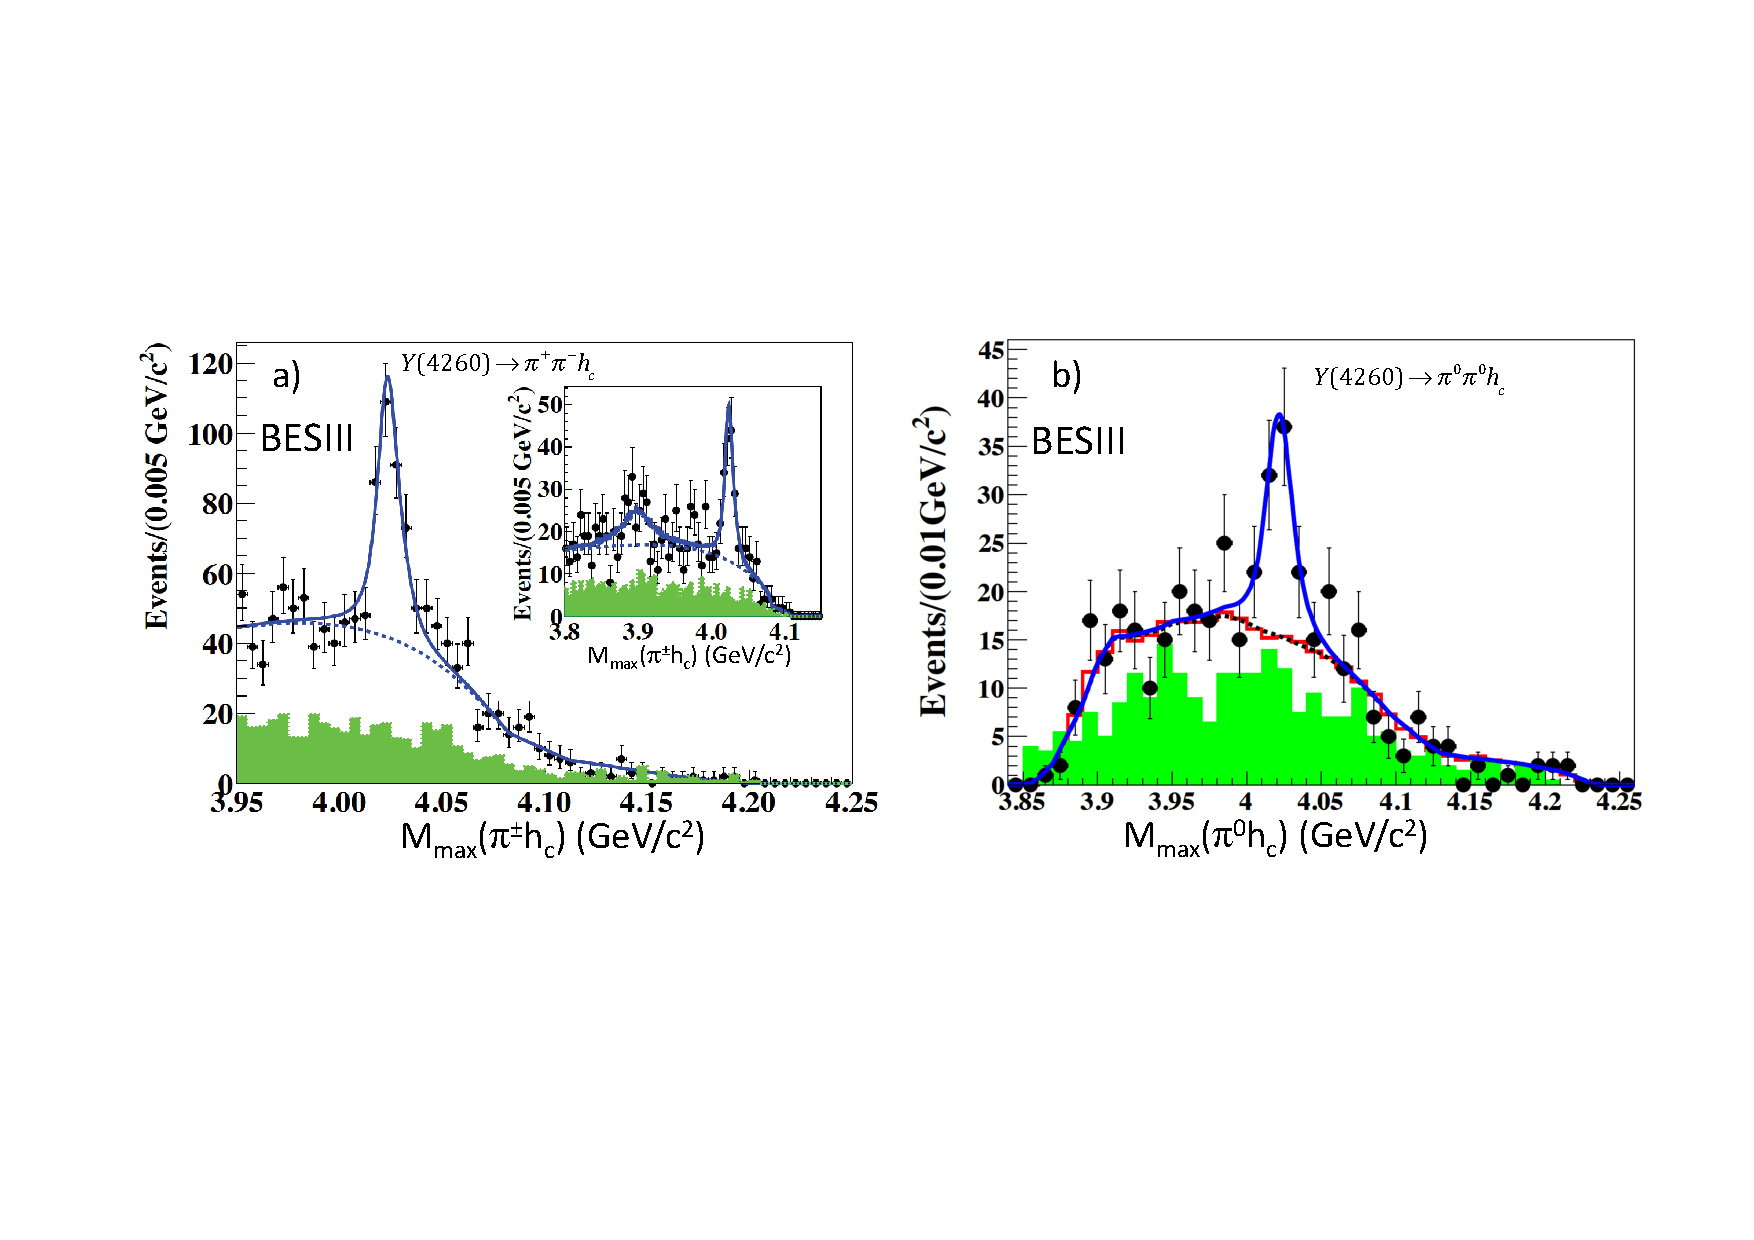
\includegraphics[width=0.95\textwidth]{Figures/01_Introduction/Exotic/charged_particle/bes3_zc4020_pihc} %
   \caption{ 
   Distribution of the larger of two $h_{c}\pi^{\pm}$ masses in $\ep\en\to h_{c}\pip\pim$ events collected in \besiii
   at $E_{cm}=4260 \mev$ and $E_{cm}=4360 \mev$\supercite{PhysRevLett.111.242001} (left),
   The $h_{c}\piz$ invariant mass distribution in $\ep\en\to h_{c}\piz\piz$ events collected in \besiii at \besiii
   \supercite{PhysRevLett.113.212002} (right)}.
\label{fig:Z4020}
\end{figure}

The theoretical pictures of $Z_c(3900)$ and $Z_c(4020)$ are not very clear yet.
For example,
the mass of these two states are in agreement with the molecular interpretation,
and both $Z_c$ states should copiously decay to $h_{c}\pi$ in a purely molecular interpretation.
But the $Z_c(4020)$ is not observed in $\jpsi\pi$
and $Z_c(3900)$ is not observed in $h_{c}\pi$.




\subsubsection{Observation of $Z_{cs}$ states}
\label{subsubsec:01_Zcs_observation}


Recently,
the \besiii experiment reported observation of the threshold structure in the $D_s^-\Dstarz+\Dssm\Dz$ mass distribution~\supercite{Ablikim:2020hsk}. 
This structure is interpreted as a resonance, 
and is named as $Z_{cs}(3985)^-$. 
The measured mass of this resonance is $3982.5_{-2.6}^{+1.8}\stat\pm2.1\syst$\mev and width is equal to $12.8_{-4.4}^{+5.3}\stat\pm3.0\syst$\mev,
and the significance of this state is around $5.3\sigma$.
The corresponding \Kp recoil-mass distributions are shown in Figure.~\ref{fig:Zcs3985},

\begin{figure}[!hbtp]
\centering
   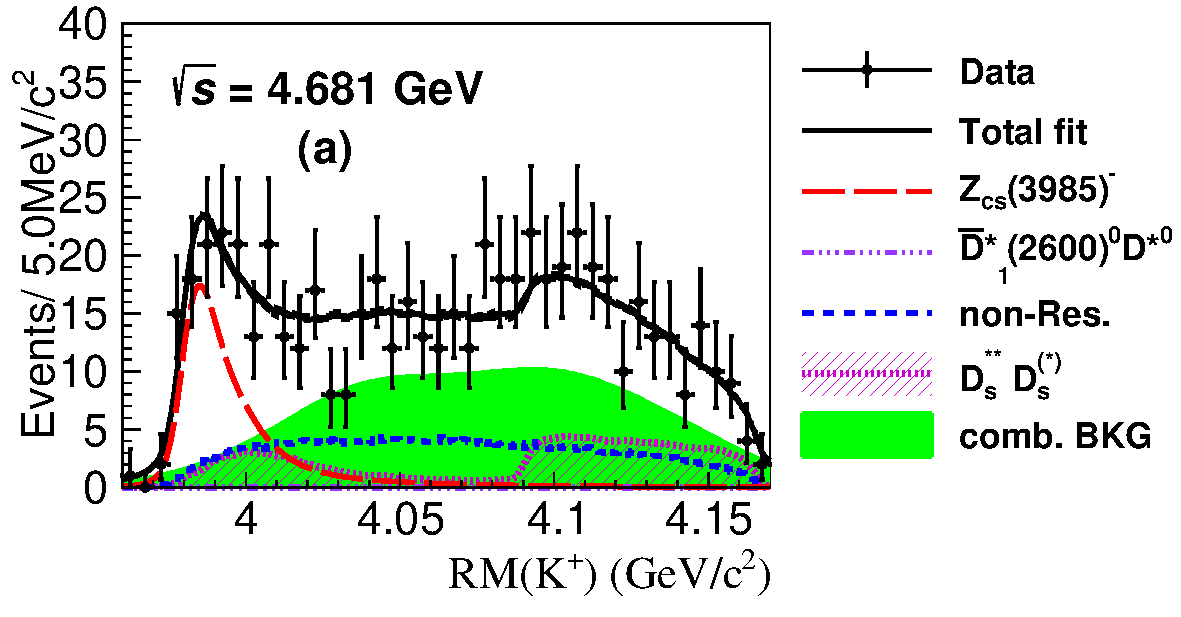
\includegraphics[width=0.51\textwidth]{Figures/01_Introduction/Exotic/Zcs/data_4680_Simulfit_withsig-eps-converted-to} %
   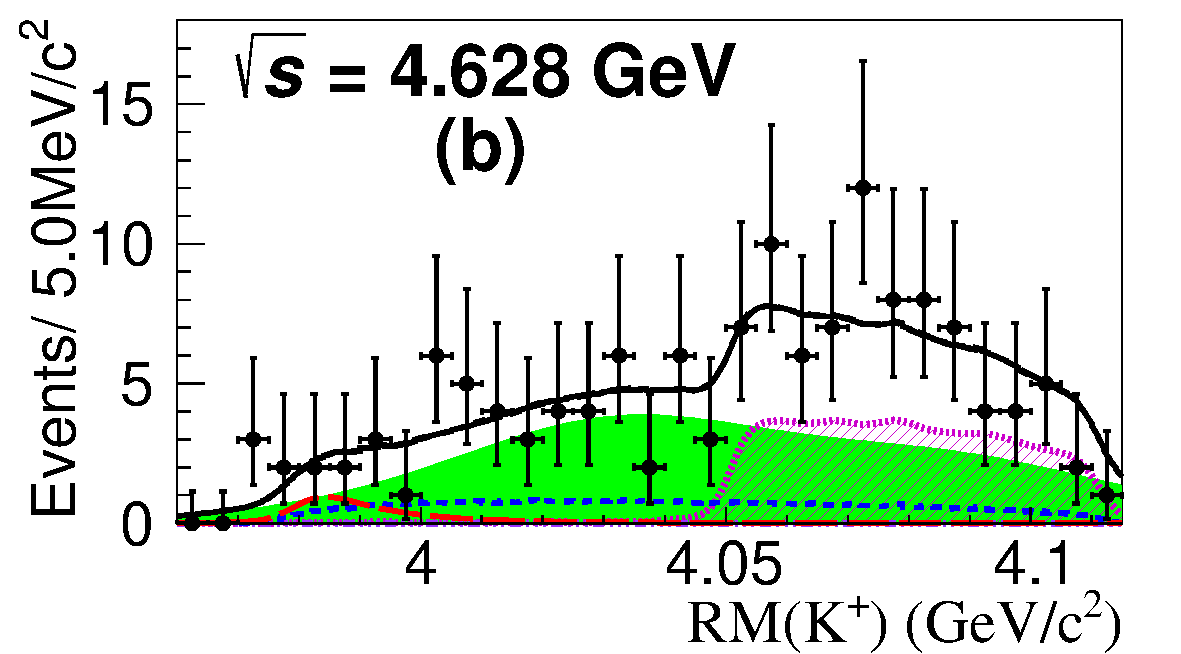
\includegraphics[width=0.48\textwidth]{Figures/01_Introduction/Exotic/Zcs/data_4626_Simulfit_withsig-eps-converted-to} %
   \caption{ 
   Simultaneous unbinned maximum likelihood fit to the \Kp recoil-mass spectra in data at 4.681 \gev (left) and 4.628 \gev (right)
   \supercite{Ablikim:2020hsk}.}
\label{fig:Zcs3985}
\end{figure}

Before the results from \besiii were reported, 
we had observed two $Z_{cs}$ states,
as well as several new $X$ states,
in $\Bp\to\jpsi\phi\Kp$ decay based on a 6-dememtional amplitude analysis at \lhcb.
The detailed analysis procedure is introduced in Chapter.~\ref{chap:Zcs_study},
and some main conclusions are illustrated here.
Figure~\ref{fig:Zcs4000_dalitz} shows the Dalitz plots for \Bp candidates in the signal region.
The most apparent features are four bands in the $\jpsi\phi$ mass distribution, 
corresponding to the previously reported $X(4140)$, $X(4274)$, $X(4500)$ and $X(4700)$ states.
There is also a distinct $\jpsi\Kp$ band near $16\gev^2$,
which is the sign of $Z_{cs}(4000)$.

\begin{figure}[!hbtp]
\centering
   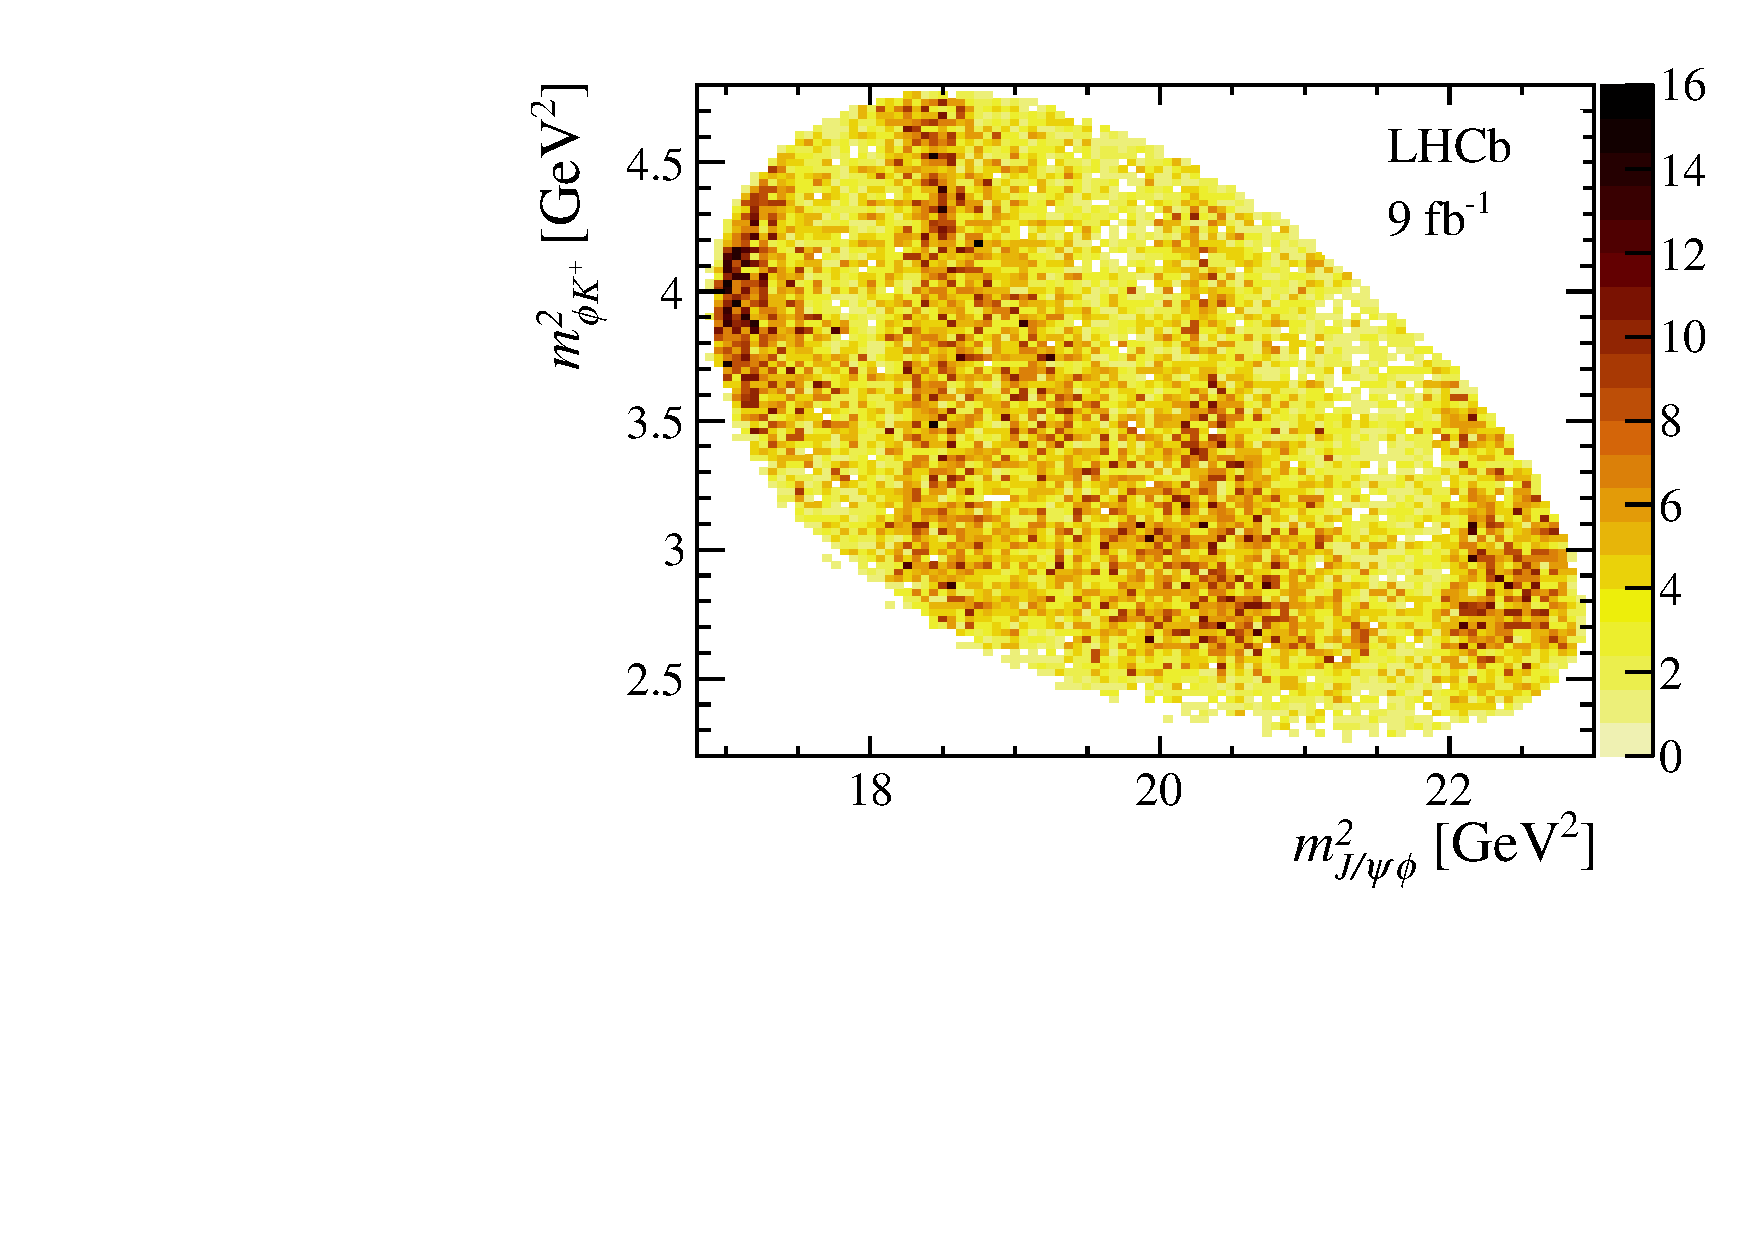
\includegraphics[width=0.45\textwidth]{Figures/01_Introduction/Exotic/Zcs/mphik2_mjpsiphi2} %
   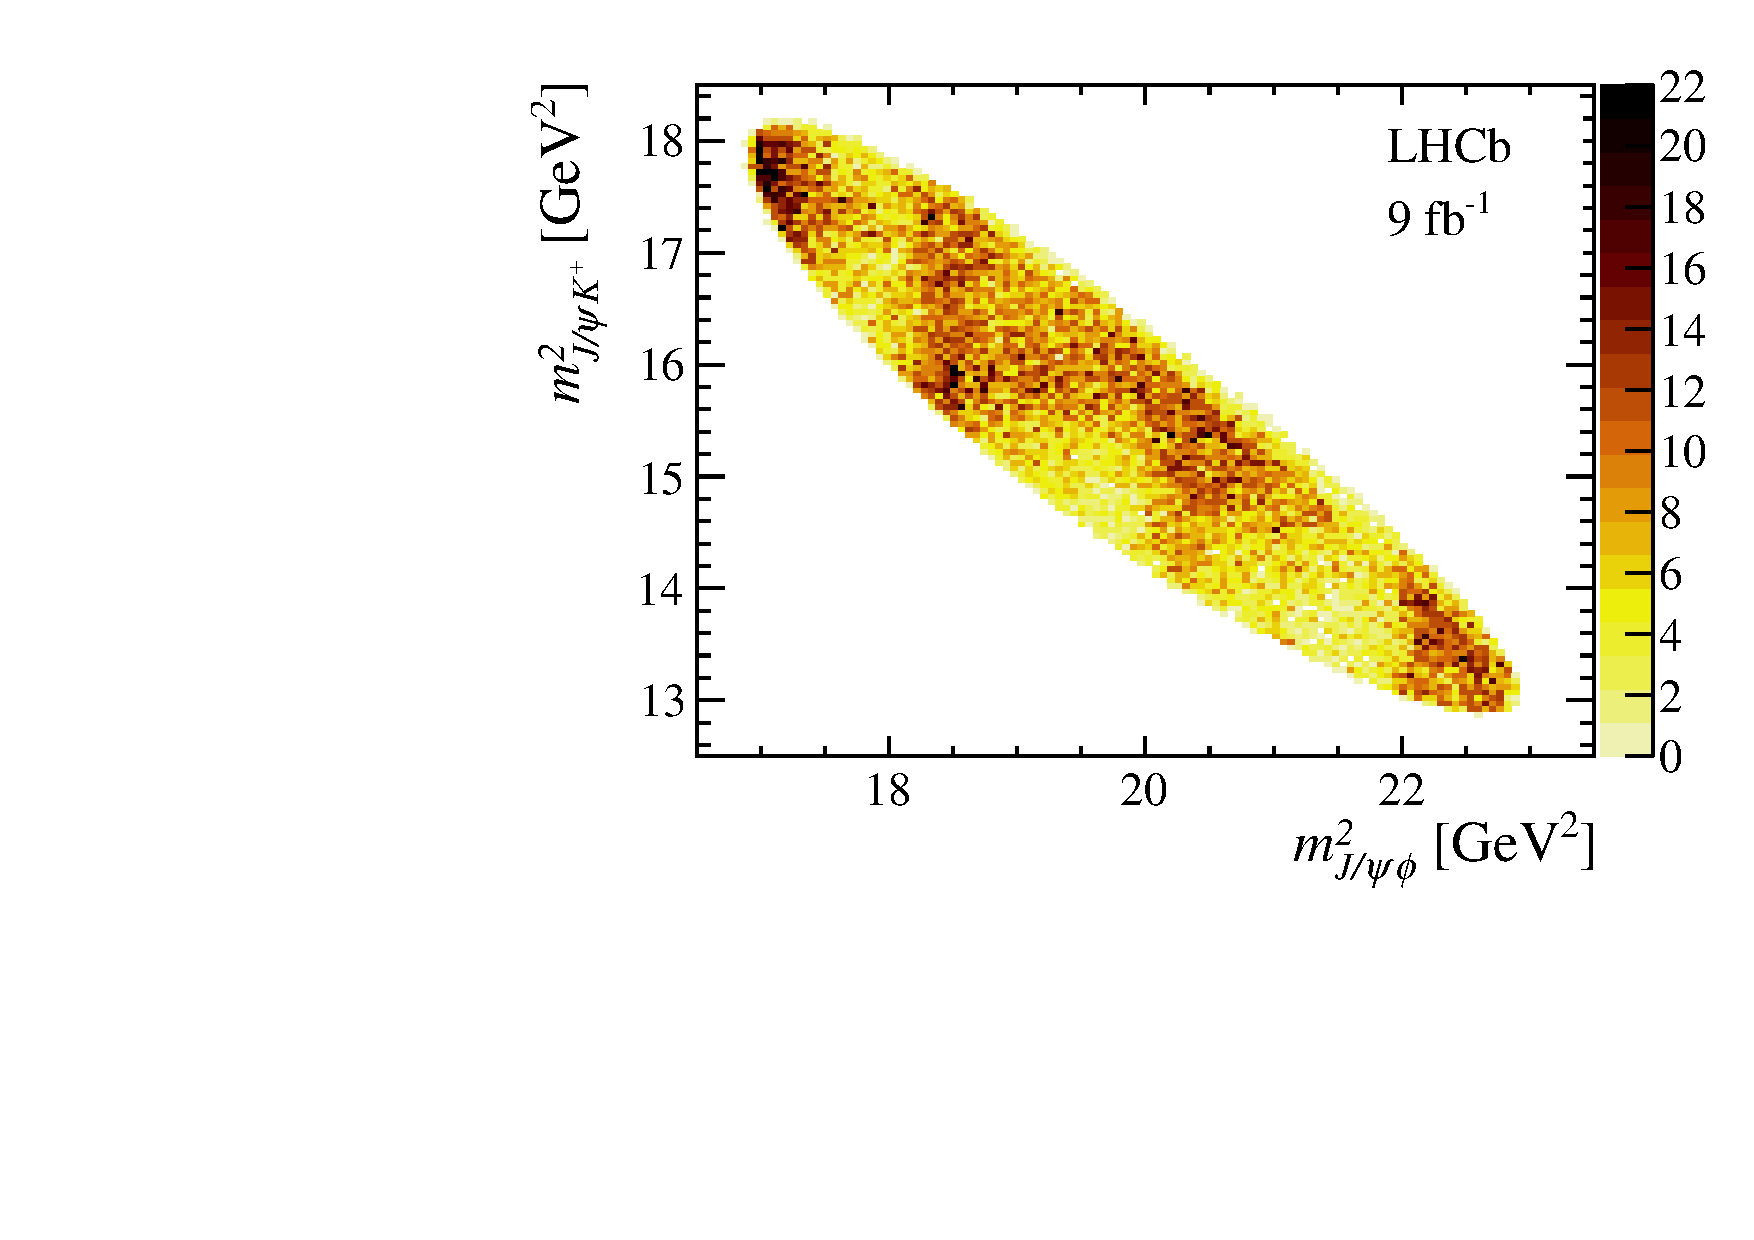
\includegraphics[width=0.45\textwidth]{Figures/01_Introduction/Exotic/Zcs/mjpsik2_mjpsiphi2} %
   \caption{ 
   Dalitz plots for $\Bu\to\jpsi\phi\Kp$ candidates in a region $\pm$15\mev around the $B^+$ mass peak.}
\label{fig:Zcs4000_dalitz}
\end{figure}

The left two plots in Figure~\ref{fig:Zcs4000} shows the $m_{\jpsi\Kp}$ distributions in two slices of $m_{\jpsi\phi}$,
which illustrates the need for the narrower $Z_{cs}(4000)^+$ state. 
Beside,
the spin and parity of $Z_{cs}(4000)$ is determined to be $1^{+}$. 
Further evidence for the resonant character of $Z_{cs}(4000)^+$ is observed in the right plot of Figure.~\ref{fig:Zcs4000}, 
showing the evolution of the complex amplitude on the Argand diagram.
The magnitude and phase exhibit approximately circular evolution with $m_{\jpsi\Kp}$ in the counter-clockwise direction,
as expected for a resonance.

We consider the $Z_{cs}(4000)$ observed at \lhcb and $Z_{cs}(3985)$ claimed by \besiii are not same state.
First, 
the width of these two states are pretty different.
Second,
we tried to fix the mass of width of $Zcs(3985)$ in $\Bp\to\jpsi\phi\Kp$ amplitude model,
but no significant likelihood improvement was obtained by this procedure. 
Considering the similar $Z_{c}(3900)$ and $Z_{c}(4020)$ have not been observed at any $B$ meson decay channel,
the production mechanism for $Z_{cs}(4000)$ and $Z_{cs}(3985)$ should be different.


\begin{figure}[!hbtp]
\centering
   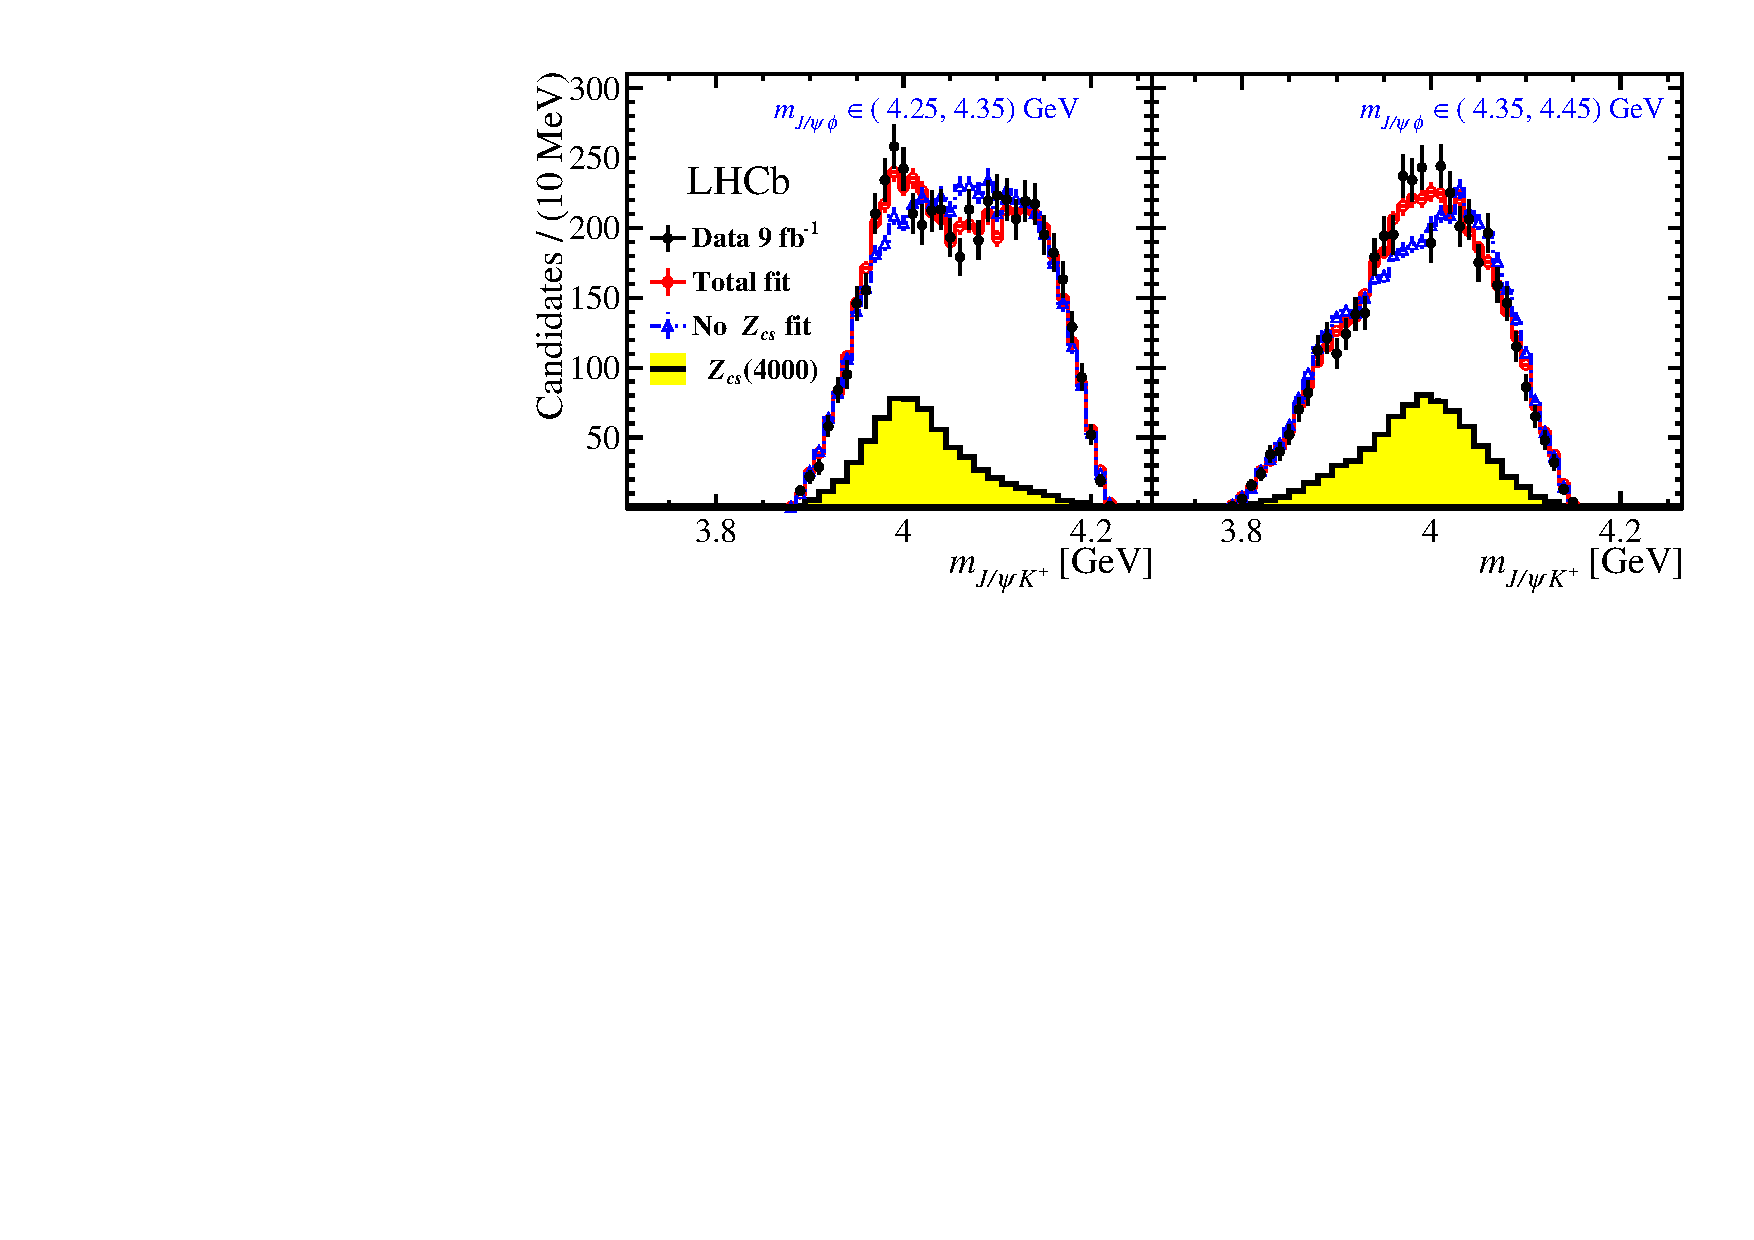
\includegraphics[width=0.65\textwidth]{Figures/01_Introduction/Exotic/Zcs/jpsik_projection} %
   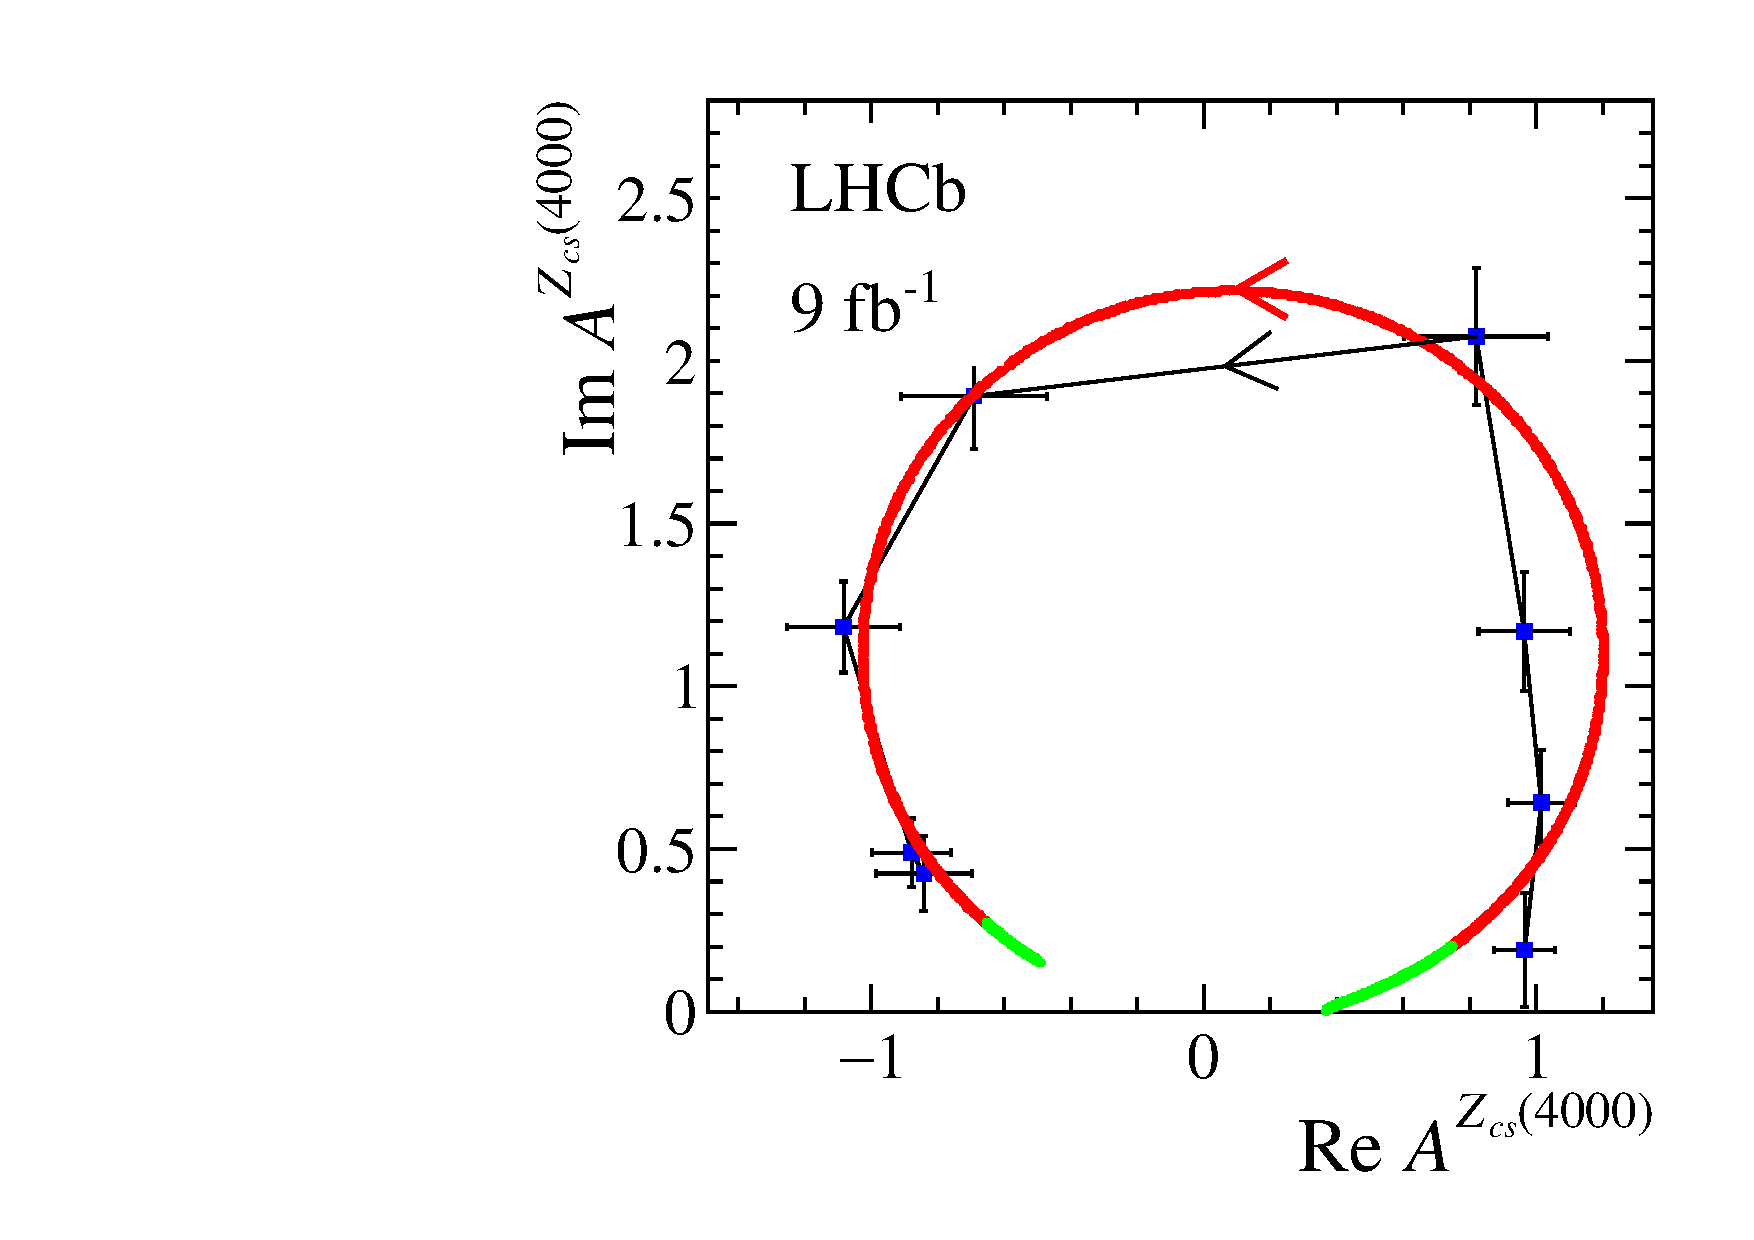
\includegraphics[width=0.325\textwidth]{Figures/01_Introduction/Exotic/Zcs/Z1_argand} %
   %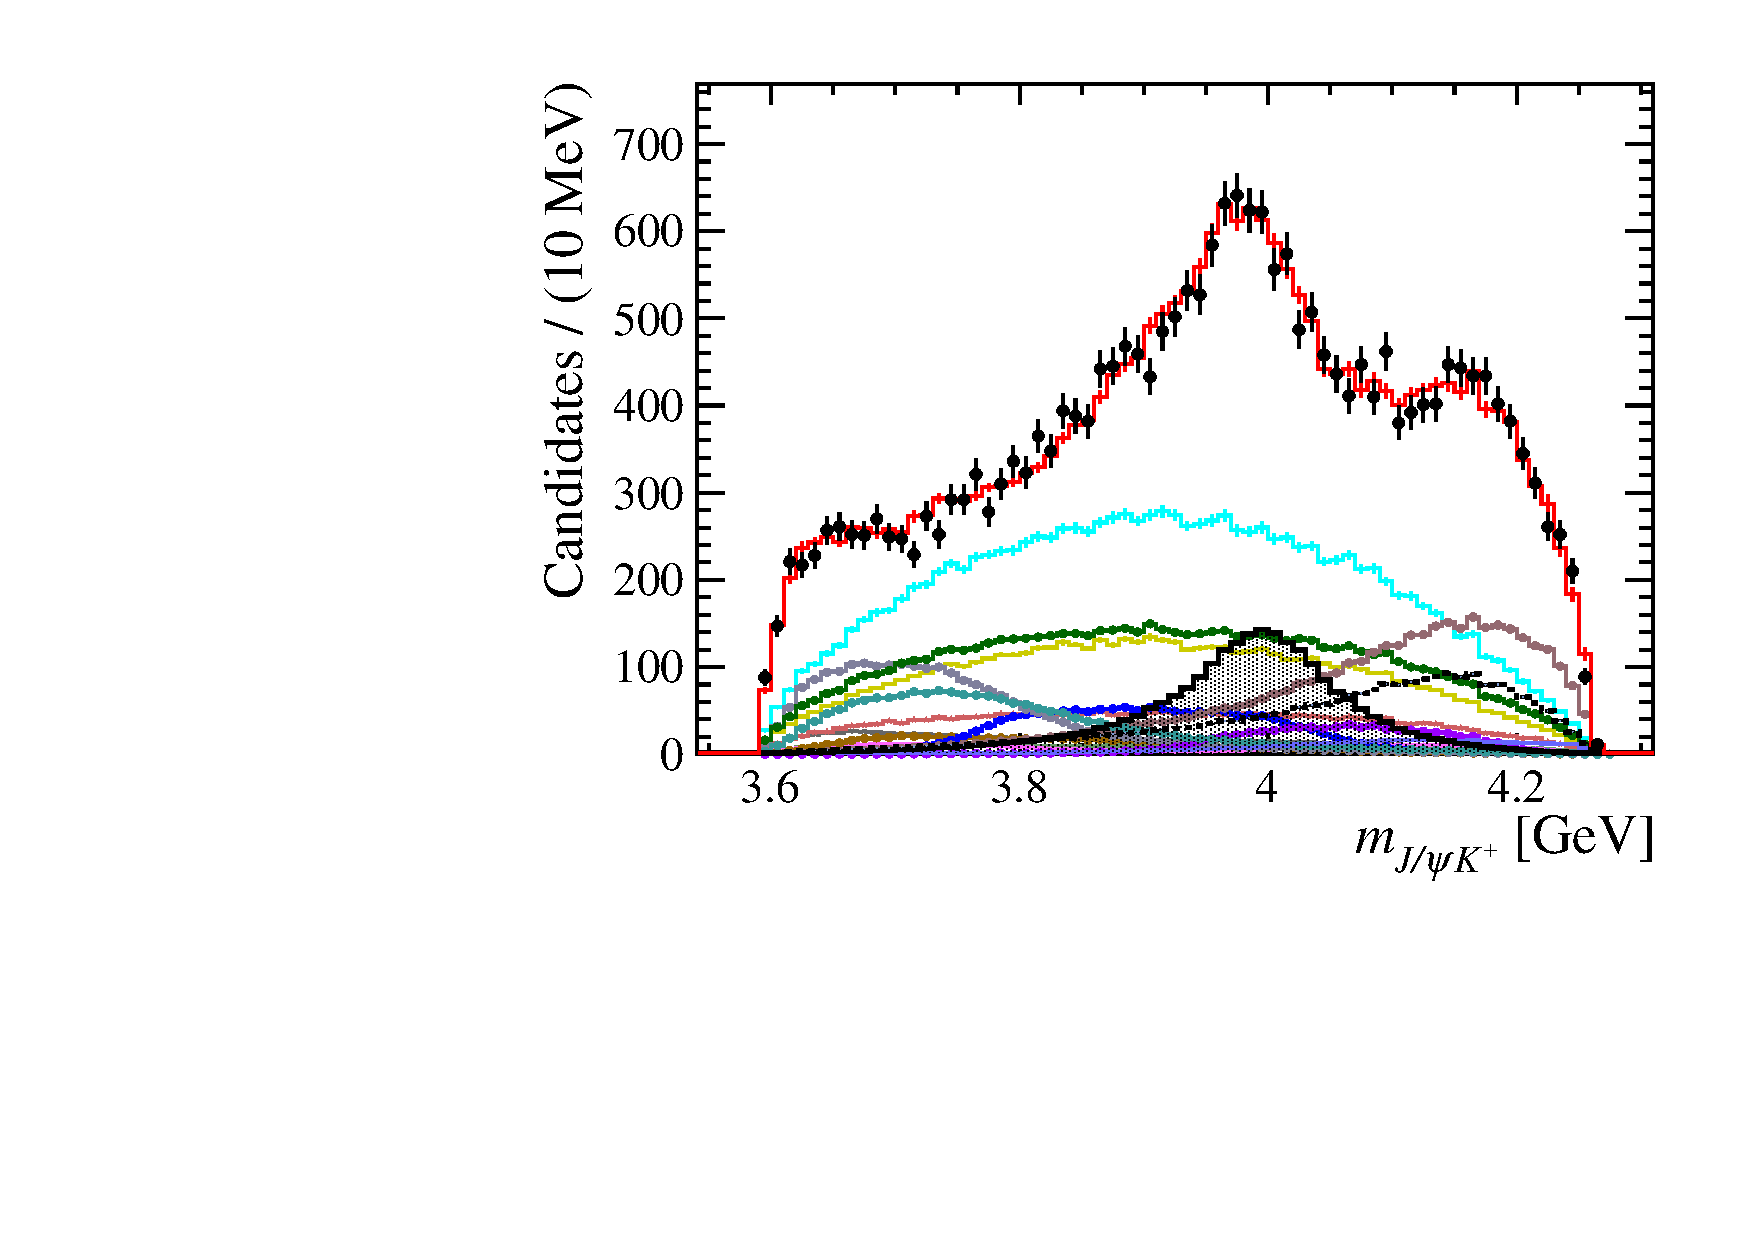
\includegraphics[width=0.4\textwidth]{Figures/01_Introduction/Exotic/Zcs/mjpsik-New} %
   \caption{
   Fit projections onto $m_{\jpsi\Kp}$ in two slices of $m_{\jpsi\phi}$ for the default model and the default model 
   without the $1^+$ $Z_{cs}$ states (left and middle) .
   Fitted values of the $Z_{cs}(4000)^+$ amplitude in eight $m_{\jpsi\Kp}$ bins,
   shown on an Argand diagram (blue points).
   The red curve represents the expected Breit-Wigner behaviour between $-1.4\Gamma_0$ to $1.4\Gamma_0$ around the $Z_{cs}(4000)^+$ mass.
   The green curve is the same as the red curve but the mass is extended to the reachable range in the $\Bp\to\jpsi\phi\Kp$ channel (right).}
\label{fig:Zcs4000}
\end{figure}

The mass thresholds of $\Ds\Dzb$ excitations, 
with S-wave $J^P$ values, 
are shown in Table~\ref{tab:mt1} and \ref{tab:mt2}.
The $Z_{cs}(4000)$ and $Z_{cs}(3985)$ are close to the thresholds 
and the S-wave $J^P$ are consistent to the results obtained from the amplitude fit. 
Higher values of angular momentum are expected to be suppressed for threshold effects.

\begin{table}[h]
\scriptsize
%\scriptsize
\begin{center}
\caption{Mass threshold and S-wave $J^P$ of $\Ds\Dzb$ containing $\ccbar u\squarkbar$.}
\label{tab:mt2}
\begin{tabular}{|c|c|c|c|}
\hline
L=0                   &\tabincell{c}{$0^-$ \Dsp \\ (1968\mev)}
&\tabincell{c}{$1^-$ \Dssp \\ (2112\mev)}             &\tabincell{c}{$0^+$ $D^{*+}_{s0}$ \\ (2318\mev)}        \\
\hline
\tabincell{c}{$0^-$ \Dz \\ (1870\mev)}                &\tabincell{c}{$0^+$ \\ (3838\mev)}
&{\color{red} \tabincell{c}{ $1^+$ \\ (3982\mev)} }   &\tabincell{c}{$0^-$  \\ (4188\mev)}   \\
\hline
\tabincell{c}{$1^-$ \Dstar \\ (2007\mev)}             &{\color{red} \tabincell{c}{$1^+$ \\ (3975\mev)} }
&\tabincell{c}{$0^+$ \\ (4119\mev)}                   &\tabincell{c}{$1^-$ \\ (4325\mev)}                  \\
\hline
\tabincell{c}{$0^+$ $D^*_0$\\(2318\mev)}              &\tabincell{c}{$0^-$   \\ (4286\mev)}
&\tabincell{c}{$1^-$ \\ (4430\mev)} &\tabincell{c}{$0^+$  \\ (4636\mev)}                \\
\hline
\end{tabular}
\end{center}
\end{table}




\subsection{Pentaquark candidates}

\lhcb reported significant $\jpsi\proton$ mass structures in $\Lb\to\jpsi\proton\Km$ decays using Run 1 data sample,
and the reflection from $\Lz^{*}\to\jpsi\Km$ contributions have 
been be excluded from full amplitude analysis\supercite{LHCb-PAPER-2015-029}.
The Dalitz plot of $\Lb\to\jpsi\proton\Km$ is shown in the left of Figure.~\ref{fig:Pc_dalitz} with Run 1 data.
%This reinforced the results from the earlier model dependent amplitude analysis of the same data\supercite{LHCb-PAPER-2015-029},
From the 6-dimentional amplitude analysis,
the $P_{c}(4450)^{+}$ structure was determined to peak at $4449.8\pm 1.7\pm 2.5$ \mev,
with a width of $39\pm 5\pm 19$ \mev.
%Even though not apparent from the $m(\jpsi\proton)$ distribution,
%the amplitude analysis required also a second,
%broad $\jpsi\proton$ state for a reasonable description of the data,
%peaking at $4380\pm 8\pm 29$ \mev,
%with a width of $205\pm18\pm86$\mev.
The amplitude analysis also required a second broad $\jpsi\proton$ state for a reasonable description of the data,
peaking at $4380\pm 8\pm 29$ \mev,
with a width of $205\pm18\pm86$\mev,
even though it did not appear in the $m(\jpsi\proton)$ distribution,
The fitting projection on $m_{\jpsi\proton}$ is shown in the left of Figure.~\ref{fig:Pc_mass}.
The spins of these structures were not determined,
and the data preferred spin combinations involving $3/2$ and $5/2$ in either order.
The spin-parity preferences exhibited significant $\Lz^{*}$ model dependence.
Investigation of the Argand diagrams for the $P_{c}(4450)^{+}$ and $P_{c}(4380)^{+}$ structures was inconclusive
because of the large statistical errors.
Then, 
cross check was performed in a nearly model independent way in Ref.~[\cite{LHCb-PAPER-2016-009}],
where it was shown that the $\jpsi\proton$ structure near 4450\mev 
was too narrow to be accounted by a collection of $\proton\kaon$ contributions.

\begin{figure}[!hbtp]
\centering
   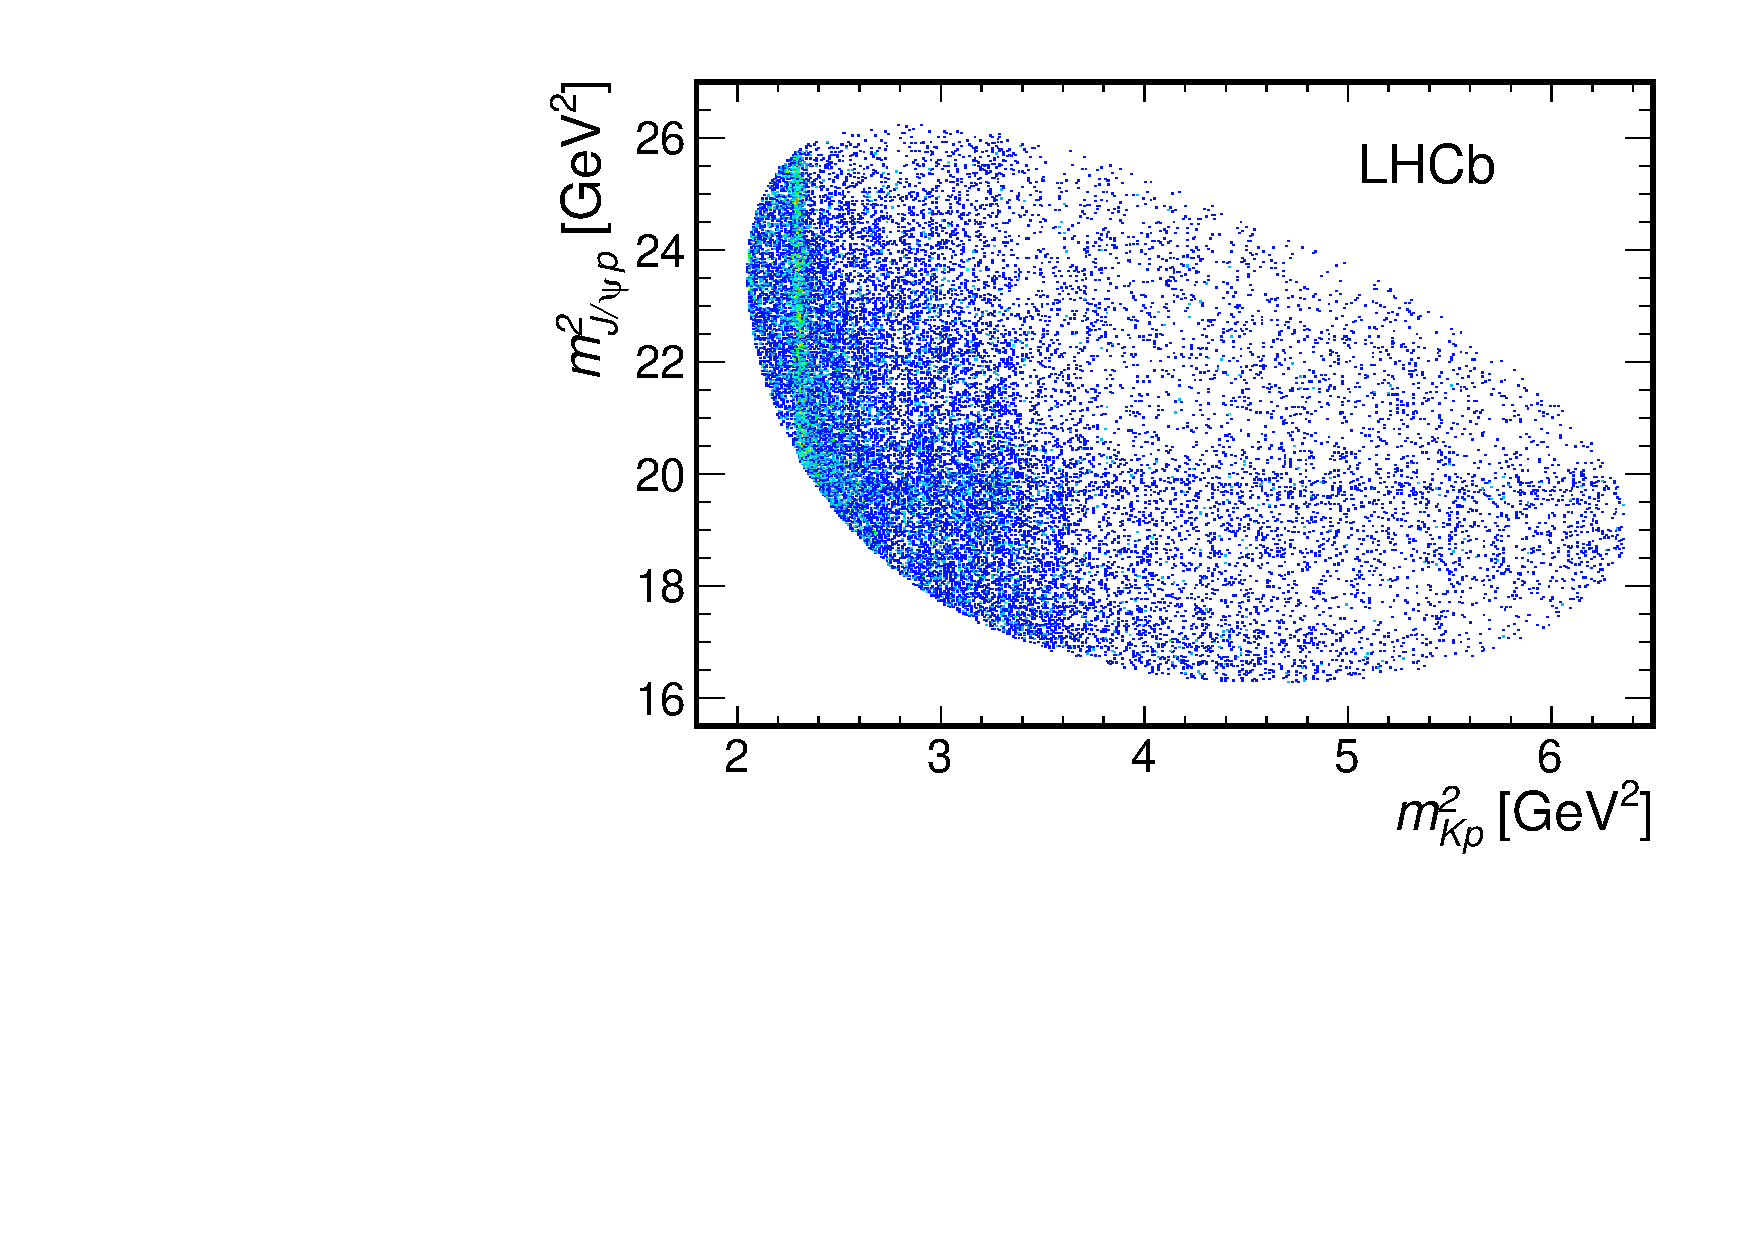
\includegraphics[width=0.48\textwidth]{Figures/01_Introduction/Exotic/Pc_states/2015-lhcb-Lb2jpsipK-dalitz} %
   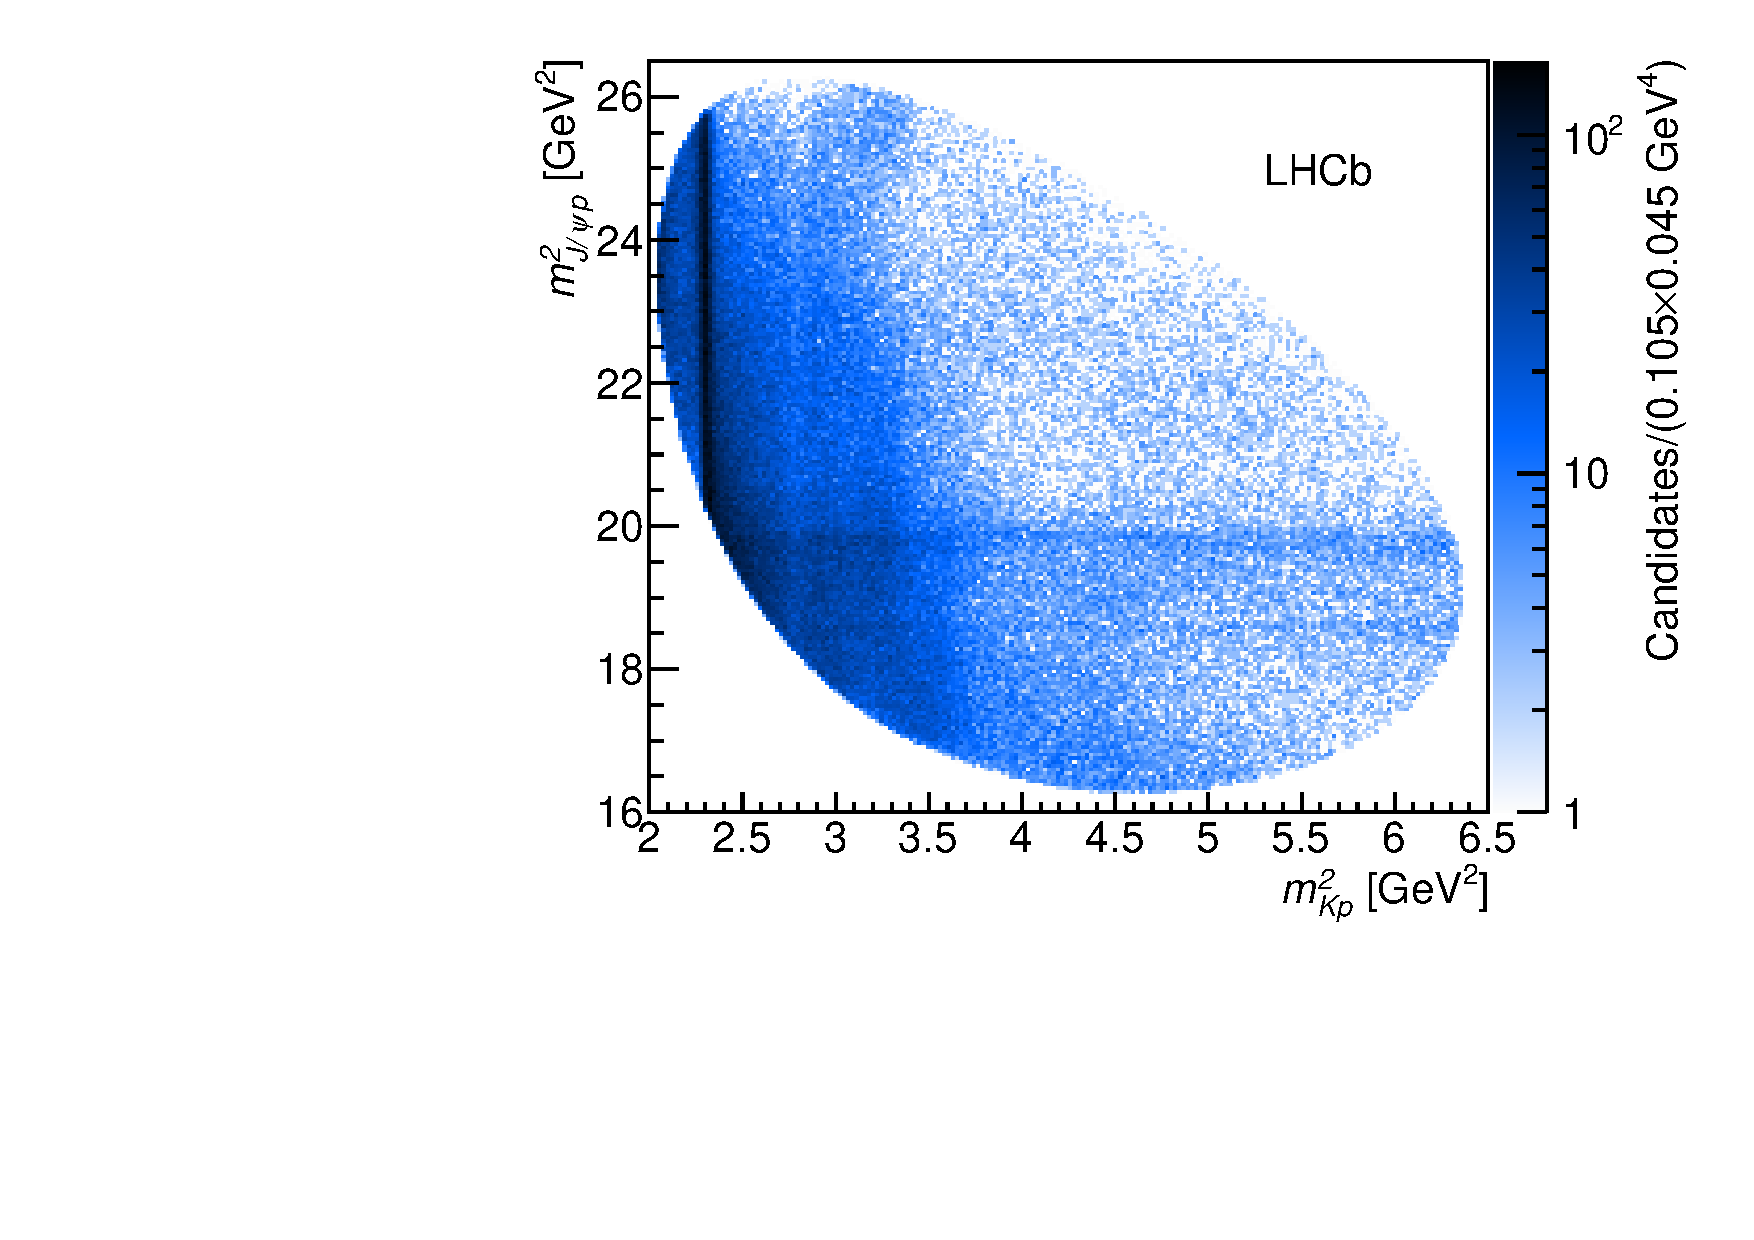
\includegraphics[width=0.43\textwidth]{Figures/01_Introduction/Exotic/Pc_states/2019-Dalitz_plot_pc} %
   \caption{ 
   Dalitz plot of $\Lb\to\jpsi\proton\Km$ with Run 1 data sample (left)\supercite{LHCb-PAPER-2015-029}, 
   with Run 1 and Run 2 data sample together (right)\supercite{LHCb-PAPER-2019-014}.}
\label{fig:Pc_dalitz}
\end{figure}

We then updated $\Lb\to\jpsi\proton\Km$ based on the combined data set collected by the \lhcb collaboration in Run 1,
with $\proton\proton$ collision energies of $7$ and $8 \tev$ corresponding to a total integral luminosity of $3 \invfb$,
and the Run 2 samples with $\proton\proton$ collision energies of $13 \tev$ corresponding to $6 \invfb$\supercite{LHCb-PAPER-2019-014}.
In this updated analysis,
the selection procedure is optimized,
which helps to improve the $\Lb$ reconstruction efficiency  by alomost a factor of two 
and leaves the background level almost unchanged,
detiails of selection procedure are introduced in Appendix.~\ref{app:pentaquark_jpsipk}.
The invariant mass distributions are consistent to the previous study according to the Dalitz plots,
as shown in Figure.~\ref{fig:Pc_dalitz}.
Besides,
performing a rigorous amplitude analysis of this new data sample is computationally challenging.
Therefore,
we applied binned fits to the 1-dimentional distribution $m_{\jpsi\proton}$ distribution,
as shown in the right of Figure.~\ref{fig:Pc_mass}.
Using the nine-fold increased $\Lb$ sample,
the previous reported $P_{c}(4450)^+$ peak is confirmed and resolved into two narrow states,
$P_{c}(4440)^+$ and $P_{c}(4457)^+$.
A narrow $P_{c}(4312)^+$ is discovered with $7.3\sigma$ significance.

Since all three states are narrow and below the $\Sigma_{c}^{+}\Dzb$ and $\Sigma_{c}^{+}\Dstarzb$ thresholds 
within plausible hadron-hadron binding energies, 
they provide the strongest experimental evidence to date for the existence of bound states of a baryon and a meson. 
According to some theorical models\supercite{PhysRev.134.B1307,PhysRevC.98.045208,MAIANI2018247,Bugg_2008,PhysRevD.91.051504},
several other $P_{c}^+$ states should exist.
We expect more structures will be observed at \lhcb with a larger data sample. 


\begin{figure}[!hbtp]
\centering
   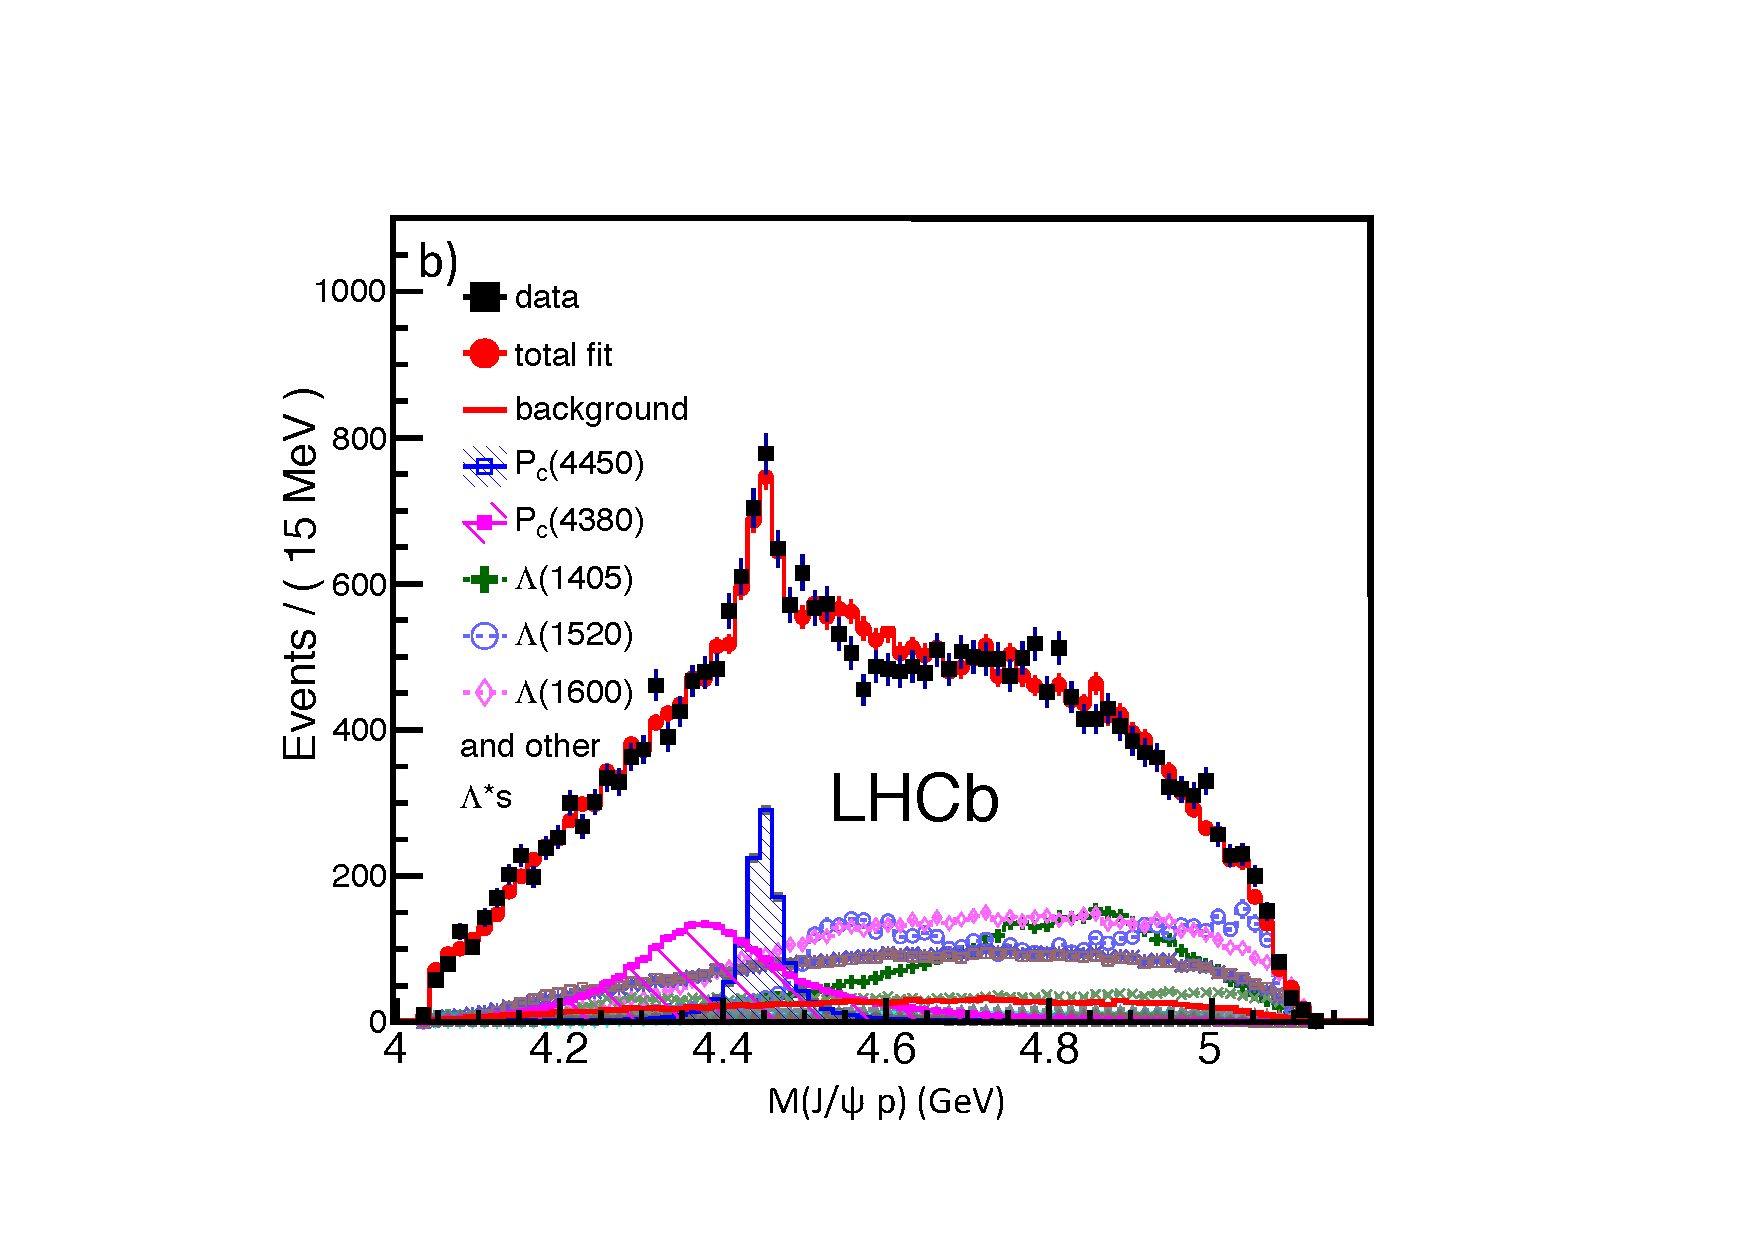
\includegraphics[width=0.46\textwidth]{Figures/01_Introduction/Exotic/Pc_states/2015-lhcb-Lb2jpsipK-mjpsip-default-slo} %
   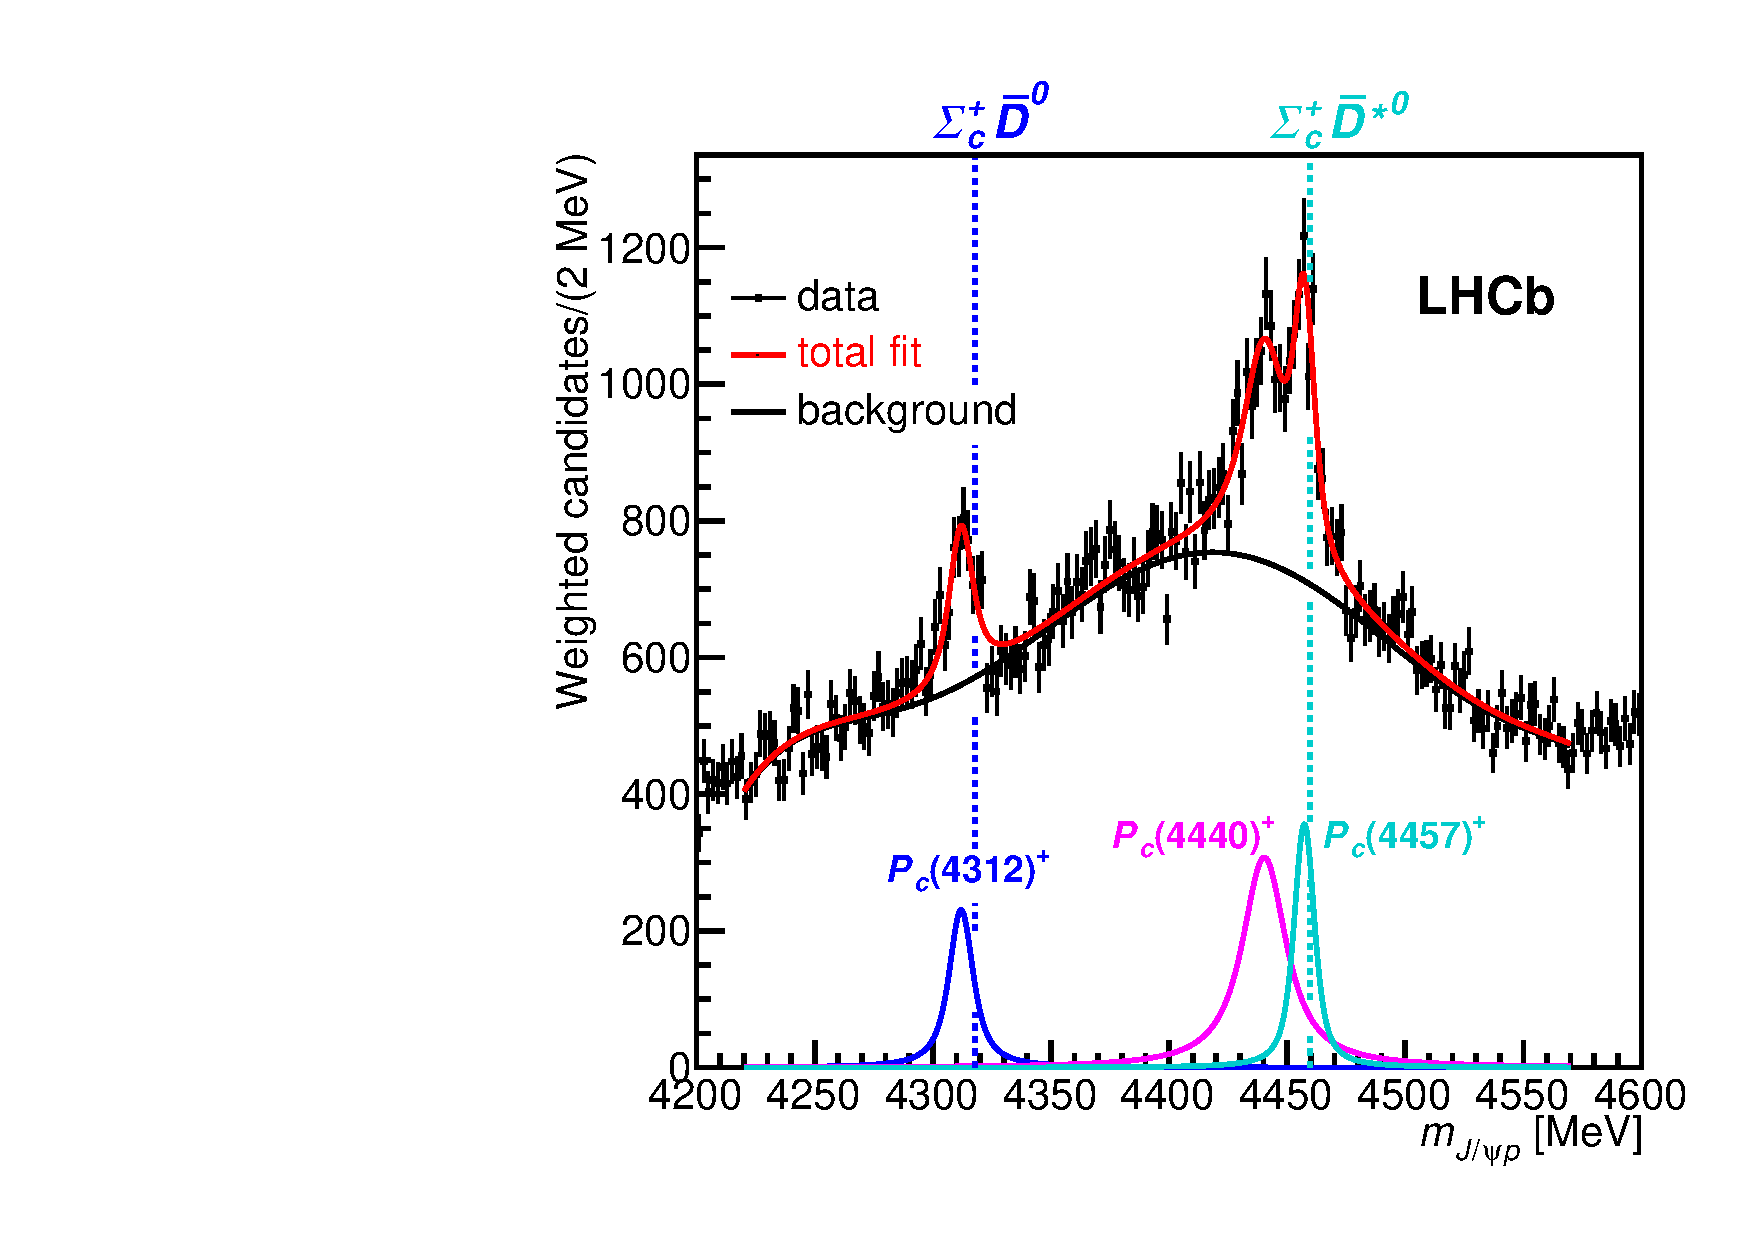
\includegraphics[width=0.44\textwidth]{Figures/01_Introduction/Exotic/Pc_states/2019-pentaquarks_nominal_fit_and_thresholds} %
   \caption{ 
   Fit projection for $m_{\jpsi\proton}$ with two $P_{c}$ states (left)\supercite{LHCb-PAPER-2015-029}.    
   Fit to $m_{\jpsi\proton}$ distribution with three BW discribed $P_{c}$ states (right)\supercite{LHCb-PAPER-2019-014}. }
\label{fig:Pc_mass}
\end{figure}

The Cabibbo-suppressed decay $\Lb\to\jpsi\proton\pim$ was also inspected at \lhcb with Run 1 sample\supercite{LHCb-PAPER-2016-015}.
From a 6-dimentional amplitude analysis,
$3.1\sigma$ evidence for summed presence of $P_{c}(4380)^+$, $P_{c}(445)^+$ and $Z_{c}(4200)^{-}$ is obtained.
The $m_{\proton\pi}$ and $m_{\jpsi\proton}$ projections of the fit are compared in Figure.~\ref{fig:Pc_jpsipi}.
Due to the ambiguities between $P_{c}^+$ and $Z_{c}^-$ terms,
any individual exotic state cannot be confirmed from this study.
Furthermore,
the previous amplitude model should be updated,
since three $P_{c}^+$ candidates are observed from the updated ananlysis at \lhcb\supercite{LHCb-PAPER-2019-014}.
We expect more significant conclusions can be obtained from the updated analysis of $\Lb\to\jpsi\proton\pim$.
The selection optimization of this channel has been finished,
and detailed progresses are introduced in Appendix.~\ref{chap:pentaquark_jpsippi}.

\begin{figure}[!hbtp]
\centering
   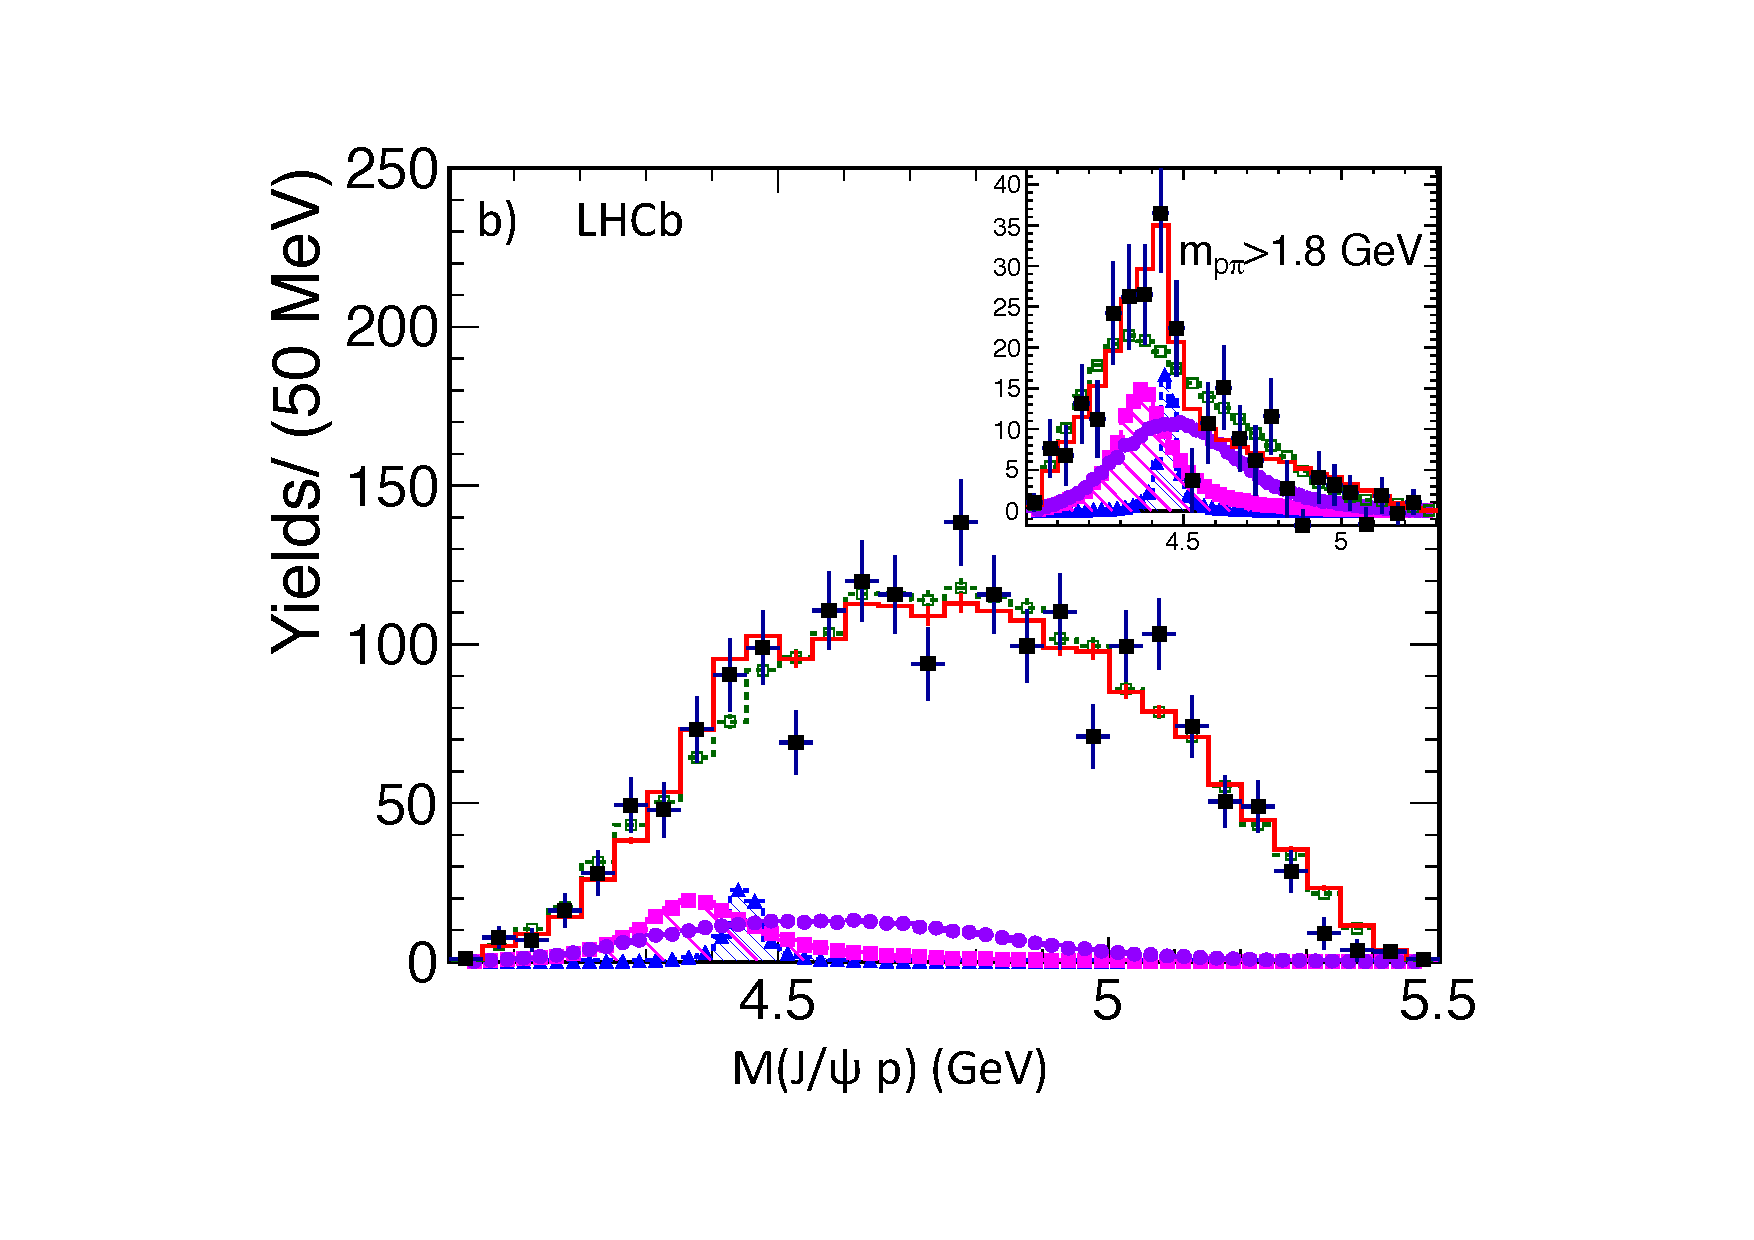
\includegraphics[width=0.45\textwidth]{Figures/01_Introduction/Exotic/Pc_states/lhcb-Lb2jpsippi-mjpsip-inset-slo} %
   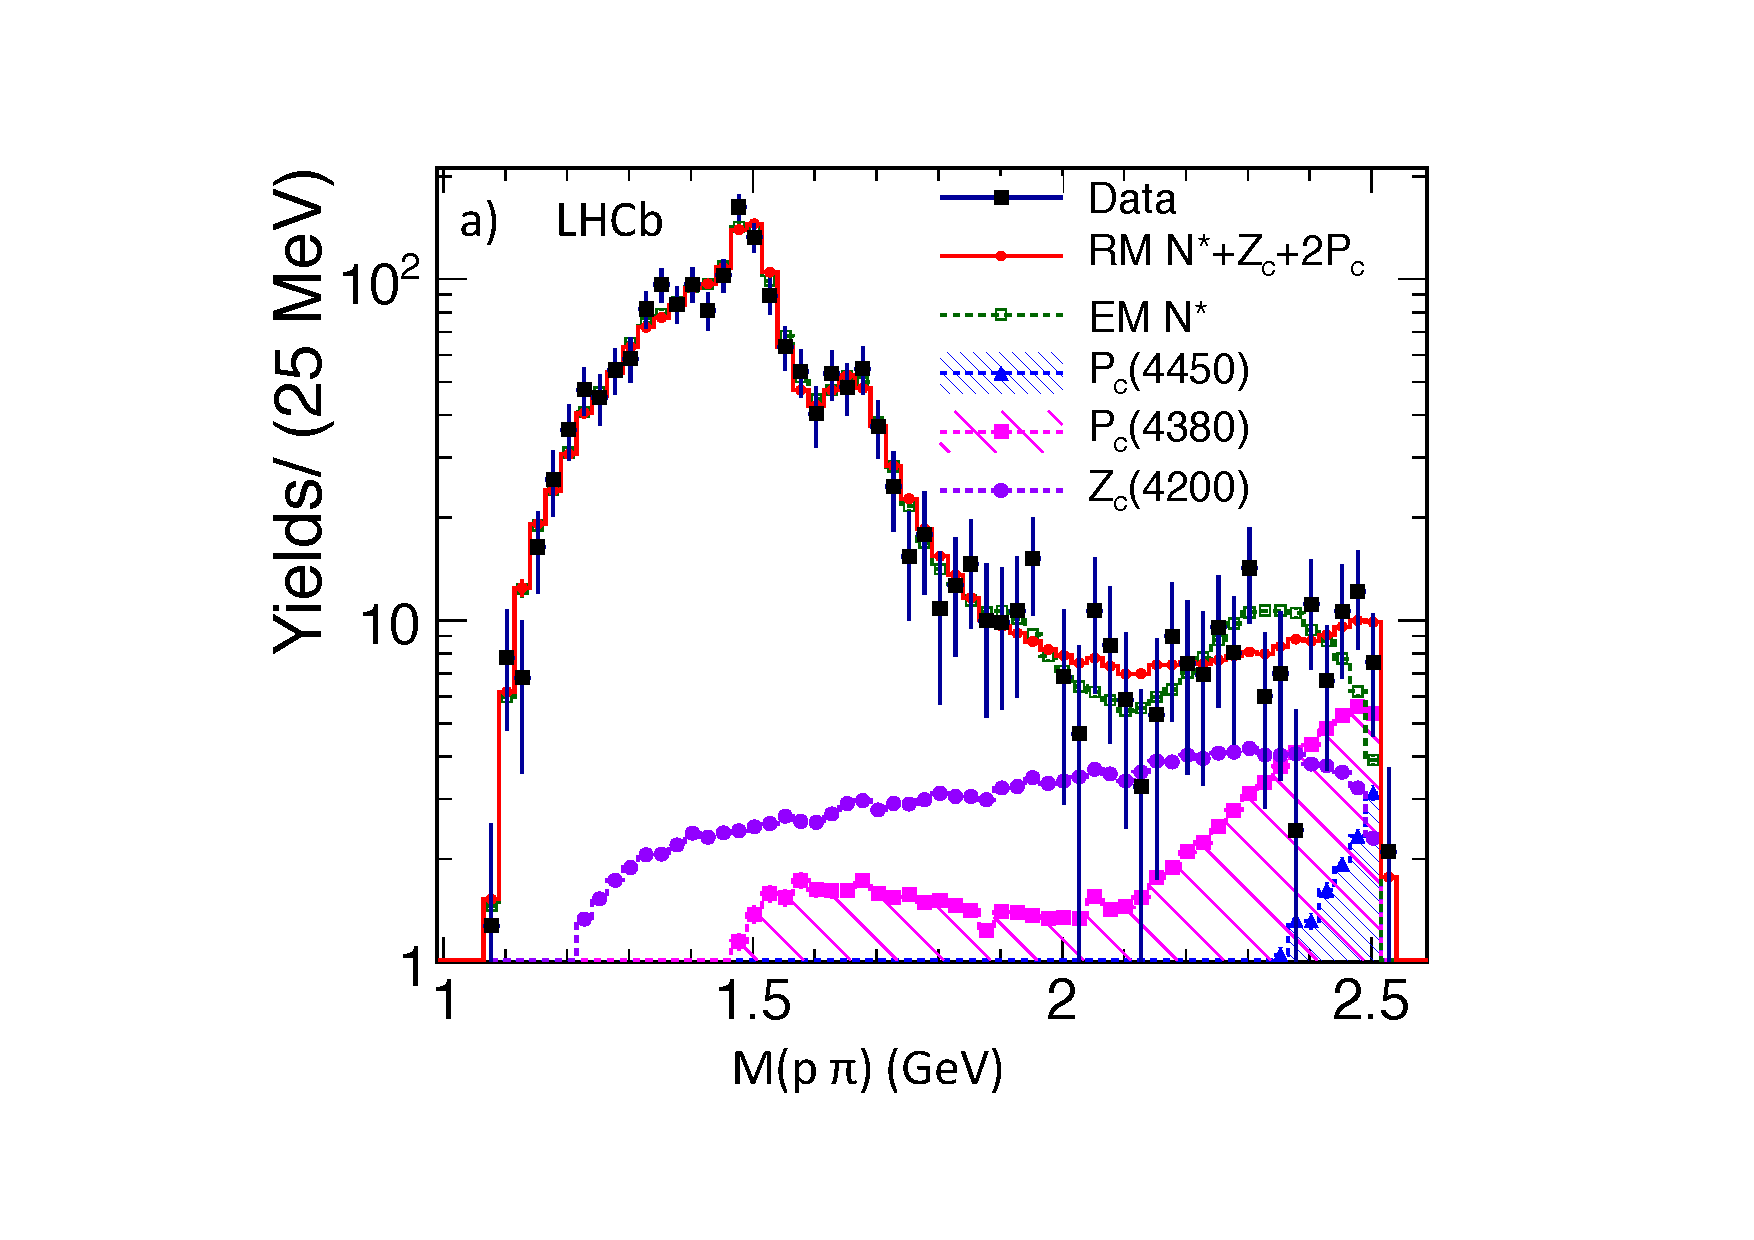
\includegraphics[width=0.44\textwidth]{Figures/01_Introduction/Exotic/Pc_states/lhcb-Lb2jpsippi-mppi-slo} %
   \caption{ 
   Projections of the amplitude fit onto $m_{\proton\pi}$ (left) and $m_{\jpsi\proton}$ data distribution for $\Lb\to\jpsi\proton\pim$ decay 
   in \lhcb\supercite{LHCb-PAPER-2016-015}.}.
\label{fig:Pc_jpsipi}
\end{figure}

The open-strange pentaquark states are searched in $\Xibm\to\jpsi\Lc\Km$ decay at \lhcb\supercite{LHCb-PAPER-2020-039},
and its significance exceeded $3\sigma$.
The $P_{cs}(4459)^0$ state has a mass only about 19 \mev below the $\Xicz\Dstarzb$
threshold and a narrow width. 
Motivated by this fact, 
the hypothesis of two resonances contributing to the enhancement is tested.
The data cannot confirm or refute the two-peak hypothesis. 

























